\documentclass[11pt,a4paper]{article}
\usepackage[hyperref]{emnlp-ijcnlp-2019}
\usepackage{times}
\usepackage{latexsym}
\usepackage{url}
%\usepackage[T1]{fontenc}

\aclfinalcopy % Uncomment this line for the final submission

%\setlength\titlebox{5cm}
% You can expand the titlebox if you need extra space
% to show all the authors. Please do not make the titlebox
% smaller than 5cm (the original size); we will check this
% in the camera-ready version and ask you to change it back.

\newcommand\BibTeX{B{\sc ib}\TeX}
\newcommand\confname{EMNLP-IJCNLP 2019}
\newcommand\conforg{SIGDAT}


\usepackage{xspace,mfirstuc,tabulary}
\newcommand{\ex}[1]{{\sf #1}}
\usepackage{graphicx}
\usepackage{tabularx}
\usepackage{array}
\newcolumntype{P}[1]{>{\centering\arraybackslash}p{#1}}
\newcolumntype{Y}{>{\raggedright\arraybackslash}X}
\newcolumntype{?}{!{\vrule width 1pt}}
\newcolumntype{h}{!{\vrule width 0.7pt}}
\usepackage[fleqn]{amsmath}
\usepackage{amsfonts}
\usepackage{algorithm2e}
\usepackage[boldmath]{numprint}
\usepackage{url}
\usepackage[caption=false,font=footnotesize]{subfig}
\usepackage{float}
%\captionsetup[subfigure]{margin=0pt}
\usepackage{booktabs}
\usepackage{tikz}
\usepackage{todonotes}

\makeatletter
\makeatother %some sort of hack related to the symbol @

\newcommand{\bs}{\boldsymbol} 
\DeclareMathOperator*{\argmax}{\arg\!\max\!} %argmax operator
\newcommand{\wrtd}{\mathrm{d}}

\newcommand{\rough}[0]{\color{purple}}

\newcommand{\Arrow}[1]{\parbox{#1}{\tikz{\draw[->](0,0)--(#1,0)}} }

%%%%%%%%%%%%%%%%%%%%%%%%%%%%%%%%%%%%%%%%%%%%%%%%%%%%%%%%%%%%%%%%%

%\title{Bayesian Ensembles of Crowds and Deep Learners for Sequence Tagging}
%Multiple Unreliable Text Annotators}
\title{A Bayesian Approach for Sequence Tagging with Crowds}

\author{Edwin Simpson and Iryna Gurevych\\
  Ubiquitous Knowledge Processing Lab \\
  Department of Computer Science \\
  Technische Universit\"at Darmstadt \\
  \url{https://www.ukp.tu-darmstadt.de} \\
  {\tt \{simpson,gurevych\}@ukp.informatik.tu-darmstadt.de}
}

\begin{document}

\maketitle

% up to eight (8) pages of content, plus unlimited pages for references
% Each EMNLP 2018 submission can be accompanied by a single PDF appendix <--put equations in here
% + one .tgz or .zip archive containing software, and one .tgz or .zip archive containing data
% make sure that these are also anonymized.

% This paper shows how common annotator models for crowdsourcing can be seen as extensions of one another
% particularly in small-data scenarios that occur at the beginning of a crowdsourcing process.
%We publish our code to encourage adaptation and reuse.
\begin{abstract}
Current methods for sequence tagging, a core task in NLP, are data hungry,
which motivates the use of crowdsourcing as a cheap way to obtain labelled data.
However, annotators are often unreliable and current aggregation methods cannot capture common types of span annotation errors.
%, as they ignore sequential dependencies between annotators' labels.
To address this, we propose a Bayesian method for aggregating sequence tags
 that reduces errors by modelling sequential dependencies between the
 annotations as well as the ground-truth labels.
By taking a Bayesian approach, we account for uncertainty in the model due to both
annotator errors and 
the lack of data for modelling annotators who complete few tasks.
We evaluate our model on crowdsourced data for named entity recognition, information extraction and argument mining,
showing that our sequential model outperforms the previous state-of-the-art. 
%and that 
%Bayesian approaches outperform non-Bayesian alternatives.
We also find that
 our approach can reduce crowdsourcing costs through
 more effective active learning, as it 
better captures uncertainty in the sequence labels when there are few annotations.
\end{abstract}

%%%%%%%%%%%%%%%%%%%%%%%%%%%%%%%%%%%%%%%%%%%%%%%%%%%%%%%%%%%%%%%%%

\section{Introduction}\label{sec:intro}

The high demand for labeled training data in current NLP methods,
particularly deep learning, is widely recognized
%with deep learning performance often improved by making use of larger training sets
\cite{zoph2016transfer, rastogi2016weighting, P14-1111}.
A common NLP task that has benefited from deep learning is \emph{sequence tagging},
which involves classifying sequences of tokens for tasks such as named entity recognition,
part-of-speech tagging, or information extraction. 
Neural network sequence taggers are typically trained on 
tens of thousands of documents %containing hundreds of thousands of tokens
~\cite{ma2016end,lample2016neural},
%This requirement for large labeled datasets 
which presents a challenge 
when facing new domains or tasks, where obtaining labels is often time-consuming or costly.
%Unlike I.I.D. classification tasks, such as document classification, the class labels in a sequence tagging task are dependent on the labels of the previous tokens.

Labeled data can be obtained cheaply by crowdsourcing, in which large
numbers of untrained workers annotate documents instead of more expensive experts.
For sequence tagging, this results in multiple sequences of unreliable labels for each document.
%Noisy labels could also be obtained from models trained on different domains,  
% multiple experts, or users of applications who click on and interact
%with text.
Probabilistic methods for aggregating these labels
have been shown to be more accurate than simple heuristics 
such as majority voting~\cite{Raykar2010,sheshadri2013square,rodrigues2013learning,hovy2013learning}.
However, work on sequence tagging is limited
and existing methods cannot model dependencies between the annotators' labels and hence 
miss error patterns such as a tendency to label overly long spans~\cite{rodrigues2014sequence,nguyen2017aggregating}.
%%%% In this paper... we develop Bayesian model for aggregating sequence labels and compare different annotator models.
In this paper, we remedy this by proposing a sequential annotator model and applying it to
 tasks that follow a \emph{beginning, inside, outside} (\emph{BIO})
 scheme, 
in which the first token in a span of type `x' is labeled `B-x',  
subsequent tokens are labeled `I-x', 
and tokens outside spans are labeled `O'.
%This results in a sequence of labels, where each label depends on its predecessor.
%We propose an aggregation method that takes advantage of the sequential dependencies between BIO tags
%to learn the reliability of individual annotators and predict the true sequence.

When learning from noisy or small datasets, commonly-used
methods based on maximum likelihood estimation may produce over-confident predictions~\cite{xiong2011bayesian,srivastava2014dropout}. 
In contrast, Bayesian inference accounts for model uncertainty when making predictions,
and enables hyperparameter tuning in unsupervised scenarios through Bayesian model selection~\cite{Bishop2006}. 
Unlike alternative methods that optimize the values for model parameters, Bayesian inference
integrates over all possible values of a parameter, weighted by a prior distribution that captures background knowledge.
The resulting posterior probabilities improve downstream decision making
as they include the probability of errors due to a lack of knowledge. For example, 
during active learning, posterior probabilities assist with selecting the most informative data points~\cite{settles2010active}.
We therefore develop a Bayesian sequence combination method, building on prior work that has demonstrated the advantages of Bayesian inference for aggregating unreliable classifications~\cite{kim2012bayesian,simpsonlong,Felt2016SemanticAA,paun2018comparing}. 
%Bayesian inference also facilitates composing a model from separate components,
%which we exploit to construct ensembles of sequence taggers and to test different annotator models.

Aggregated label quality can be improved by modeling the text features as well as the annotators~\cite{simpson2015language,Felt2016SemanticAA}.
%e.g. when performing active learning. 
For complex tasks such as sequence tagging, 
we may wish to exploit existing state-of-the-art models, such as neural networks
that do not account for model uncertainty.
%potentially forming an ensemble of multiple methods to boost performance.
In this paper, we show how to integrate existing black box methods into the aggregation model 
to construct ensembles of deep learners and human annotators. 
Our method learns the reliability of each black box method
%since they may not always perform well, particularly given small training datasets,
and avoids the need to aggregate crowdsourced data using a separate pre-processing step 
before training a sequence tagger.

% Bayesian methods have successfully been applied to various crowdsourcing tasks in NLP, such as
% sentence fragment classification~\cite{fang2014active},
% sentiment analysis~\cite{levenberg2014predicting,venanzi2014community},
% intent classification~\cite{yang2018leveraging}
% and argument ranking~\cite{simpson2018finding}, 
% but have not been adapted to sequence tagging. 

% Conversely, the methods proposed for sequence tagging
% \cite{rodrigues2014sequence,nguyen2017aggregating} do not use a fully Bayesian approach.
% We introduce a fully Bayesian approach for aggregating sequence tags from multiple sources and  
% providing a modular inference method using variational Bayes that facilitates modifications to the model.
%

% Slight re-emphasis on the black-box integration: we adapt an existing idea, and show that it works but only
% once enough crowdsourced data is obtained. So our contribution is more about evaluating an existing idea
% with a tweak that should help performance by combining two existing ideas (the reliability model with the integrated learning using EM). Less about presenting a finished, robust method.
% This needs some error analysis -- what are the confusion matrices learned for the seq tagger? E.g. do they
% successfully capture reliability of it, or do they collapse?
This paper provides the following contributions:
\begin{itemize}
 \item We propose \emph{Bayesian sequence combination (BSC)}, 
 a method for aggregating sequence labels from multiple annotators 
 that models sequential dependencies between tags 
 \item A technique for wrapping existing black-box sequence taggers into the aggregation model to improve 
 the quality of aggregated labels
 \item Theoretical and empirical comparisons of annotator models 
  for sequence tagging, including a novel model that captures sequential dependencies between annotations (referred to later as \emph{seq})
\end{itemize}
The following sections discuss related work, 
annotator models for sequence tagging,
our BSC model, and our variational inference approach
 that enables us to integrate existing sequence taggers. 
Then, we evaluate a range of Bayesian and non-Bayesian aggregation methods
with simulated annotators and two crowdsourced NLP datasets,
showing that our sequential model consistently outperforms the previous state-of-the-art,
%Our results show the benefits of a sequential annotator model and of
and benefits from the inclusion of automated sequence taggers.
% in an ensemble with human annotators.
%Our experiments evaluate both active and passive learning scenarios with varying dataset sizes, 
%analyze types of errors, and visualize the annotator models learned by our method.
We make 
%the modular implementation of our proposed method freely available, along with 
all of our code freely available\footnote{\url{http://github.com/\iftaclpubformat ukplab/arxiv2018-bayesian-ensembles\else ******\fi}}.

\subsection{Related Work}
%A number of works have investigated methods for aggregating non-sequential
%classifications from crowds.
Sheshadri and Lease~\shortcite{sheshadri2013square} benchmarked several 
aggregation models for non-sequential classifications, 
obtaining the most consistent performance from 
that of Raykar et al.~\shortcite{Raykar2010}, who
model the reliability of individual annotators
using probabilistic confusion matrices,
as proposed by Dawid and Skene~\shortcite{dawid_maximum_1979}.
%Nguyen et al.~\shortcite{hung2013evaluation} 
Simpson et al.~\shortcite{simpsonlong} showed that a Bayesian variant of of Dawid and Skene~\shortcite{dawid_maximum_1979}'s model, independent Bayesian classifier combination
(\emph{IBCC}) ~\cite{kim2012bayesian} 
can outperform maximum likelihood approaches and simple heuristics
when combining crowds of image annotators.
To reduce the number of parameters in multi-class problems,
Hovy et al.~\shortcite{hovy2013learning} proposed \emph{MACE}, 
and showed that it performed better under a Bayesian treatment on NLP tasks.
Paun et al.~\shortcite{paun2018comparing} further illustrated
the advantages of Bayesian models of annotator ability on NLP classification tasks
with different levels of annotation sparsity and noise.
We expand this work by detailing the relationships between several annotator models
and extending them to sequential classification. 
% Could we mention this: The uncertainty in such inferences may then be
% used in applications such as jointly training clas-
% sifiers (Smyth et al., 1995; Raykar et al., 2010),
% comparing crowdsourcing systems (Lease and
% Kazai, 2011), or characterizing corpus accuracy
% (Passonneau and Carpenter, 2014).
% (OR maybe mention it in the intro paragraph).
% For classification tasks in NLP, 
%  evaluated six Bayesian methods,
% % pooled model -- assumes equal annotators but allows noise
% % DS, or rather my IBCC
% % MACE
% % hierarchical DS, basically original IBCC with pooled priors
% % item difficulty model, which ignores annotator reliability
% % logrndeff, item difficulty and annotator ability
% % Bayesian: uses Hamilonian Monte Carlo
% for their ability to obtain gold labels from crowdsourced data, model annotators and item difficulty.
% They found that...
% \cite{}. 
Here we focus on the core annotator representation, rather than extensions 
for clustering annotators~\cite{venanzi2014community,moreno_bayesian_2015},
modeling their dynamics~\cite{simpsonlong},
adapting to task difficulty~\cite{whitehill2009whose,bachrach2012grade},
or time spent~\cite{venanzi2016time}.

%Previous works have applied crowdsourcing to sequence labeling tasks such as named entity recognition~\cite{ritter2011named}
%and POS-tagging~\cite{hovy2014experiments}, but these do not develop new aggregation methods.
To accout for disagreement between annotators when training a sequence tagger, Plank et al. ~\shortcite{plank2014learning} 
modify the loss function of the learner.
%to account for confusion between labels. 
However, typical cross entropy loss
naturally accommodates probabilities of labels as well as discrete labels~\cite{bekker2016training}.
%so it is unnecessary to adapt the loss function if  
%probabilities of training labels are used to account for disagreement between 
%multiple annotators
A contrasting approach is \emph{CRF-MA}~\cite{rodrigues2014sequence},
a CRF-based model that assumes only one annotator is correct for any given label.
Recently, Nguyen et al.~\shortcite{nguyen2017aggregating} proposed a hidden Markov model (HMM) approach that outperformed CRF-MA, called \emph{HMM-crowd}.
%HMM-crowd models the distribution of text tokens conditioned on the hidden state.
%More sophisticated LSTM-based sequence taggers must be trained separately given the true labels estimated by HMM-crowd.
Both CRF-MA and HMM-crowd use simpler annotator models than Dawid and Skene~\shortcite{dawid_maximum_1979}
that do not capture the effect of sequential dependencies on annotator reliability.
Neither CRF-MA nor HMM-crowd use a fully Bayesian approach.
%which has been shown to be effective for handling uncertainty
%due to noise in crowdsourced data for non-sequential classification~
%\cite{kim2012bayesian,simpsonlong,venanzi2014community,moreno_bayesian_2015}.
In this paper, we develop a sequential annotator model and a fully Bayesian method for aggregating sequence labels.  %that improves performance over previous approaches.

While HMM-crowd uses only a simple conditional independence model of text features,
Nguyen et al.~\shortcite{nguyen2017aggregating} and 
Rodrigues and Pereira~\shortcite{rodrigues2018deep} also train 
neural network sequence taggers directly on crowdsourced data
by adding a layer to handle worker reliability.
However, the proposed approaches did not outperform either CRF-MA~\cite{rodrigues2018deep} or HMM-crowd~\cite{nguyen2017aggregating}. 
A similar approach by Albarqouni et al.~\shortcite{albarqouni2016aggnet}
integrates a CNN classifier for image annotation
into an aggregation method based on 
expectation maximization (EM)~\cite{dempster_maximum_1977}.
% % While this approach improves the CNN performance over using a separate pre-processing step, 
% % their method cannot model label dependencies in sequence tagging.
Yang et al.~\shortcite{yang2018leveraging}  
adapt a Bayesian neural network so that it can be trained concurrently with an annotator model, also using EM. 
In contrast to previous work,
we do not require neural networks to be adapted, 
nor assume that their predictions are reliable 
when aggregating annotations.
Instead, we propose to learn the reliability of  
existing sequence taggers,
% using a variational approach, 
allowing untrusted, off-the-shelf taggers to enhance the performance of
the aggregation method. 

%
% takes as input only the crowdsourced labels 
%and not the features of data points~\cite{yan2011,chen2013},
%other methods improves performance by expanding 
% Their work follows earlier research on active learning from crowds that uses simpler 
% models of independent data points~\cite{fang2014active,simpson2015bayesian}. 

\section{ Modeling Sequential Annotators }\label{sec:annomodels}

When combining multiple annotators with varying skill levels, we can improve performance by modeling their individual reliability. Here, we describe several existing models 
that do not consider dependencies between annotations in a sequence,
then provide an extension that captures sequential dependencies. Each of the approaches presented employs a particular function, $A$, to model the likelihood of the annotator choosing the label $c_{\tau}$
given the true label, $t_{\tau}$, for token $\tau$.

\textbf{Accuracy model (acc)}: simply models the annotator's accuracy, $\pi$, as follows: 
\begin{flalign}
 & A = p( c_{\tau} \! = \! i | t_{\tau} \! = \! j, \pi ) = \left.
\begin{cases}
  \pi  \!&\!\!\!\text{ where } i = j \\
  \frac{1 - \pi}{J-1} \!&\!\!\!\text{ otherwise}
\end{cases} 
\right\} \!, &&
\end{flalign}
where $c_{\tau}$ is the label given by the annotator for token $\tau$, $t_{\tau}$ is its true label
and $J$ is the number of classes.
This is the basis of several previous methods~\cite{donmez2010probabilistic,rodrigues2013learning}. 
%The limitation of this approach is that it
It assumes reliability is constant,
which means that when one class label is far more common than others, 
a spammer who always selects the most common label will nonetheless 
have a high $\pi$.
%despite their labels being uninformative.
%Annotator models define a likelihood... 
%\begin{flalign}
%& A = p(c_{\tau}, c_{\tau-1}, t_{\tau}) = p( c_{\tau} \!\!=\! i | c_{\tau-1}, t_{\tau} \!=\! j, \bs\pi ),&&
%\end{flalign}

\textbf{MACE spamming model}~\cite{hovy2013learning}:
assumes a constant annotator accuracy, $\pi$,
but that when annotators are incorrect, they label according to 
a spamming distribution, $\bs\xi$, that is independent of the true label, $t_{\tau}$.
\begin{flalign}
A & = p( c_{\tau} = i | t_{\tau} = j, \pi, \bs\xi) && \nonumber \\
& = \left.
\begin{cases}
  \pi + (1 - \pi) \xi_j  &\text{ where } i = j \\
  (1 - \pi) \xi_j &\text{ otherwise}
\end{cases} 
\right\}.
\end{flalign}
This addresses the case where spammers choose the most common label when the classes are imbalanced.
While MACE can capture spamming patterns, it does not explicitly model 
different rates of errors per class. This could be an issue for sequence tagging using the 
BIO encoding, for example, if an annotator frequently labels longer spans
 than the true spans by starting the spans early. In this 
 case, they may more frequently
mis-label the `B' tokens than the `I' or `O' tokens,  which cannot be modeled by MACE. 

\textbf{Confusion vector (CV)}: this approach learns a separate accuracy 
 for each class label~\cite{nguyen2017aggregating}
using parameter vector, $\bs\pi$, of size $J$:
\begin{flalign}
& A = p( c_{\tau} \!\!=\! i | t_{\tau} \!=\! j, \bs\pi ) = \left.
\begin{cases}
  \pi_j  \!\!\!\!\!\!&\text{ where } i \!=\! j \\
  \frac{1 \!- \!\pi_j}{J-1} \!\!\!\!\!\!&\text{ otherwise}
\end{cases} 
\! \right\} \!.&&
\end{flalign}
%For the incorrect label cases where $i \! \neq \! j$,
% $p( c_{\tau} \!\!=\! i | t_{\tau} \!=\! j, \bs\pi )$ is constant for all values of $i$.
% Therefore, t
This model does not explicitly capture spamming
patterns where one of the incorrect labels has a much higher likelihood than the others.

\textbf{Confusion matrix (CM)}~\cite{dawid_maximum_1979}:
this model can be seen as an expansion of the confusion vector so that $\bs\pi$ becomes a 
$J\times J$ matrix with values given by:
\begin{flalign}
& A = p( c_{\tau} \!\!=\! i | t_{\tau} \!=\! j, \bs\pi ) = 
  \pi_{j,i} .&&
\end{flalign}
This requires a larger number of parameters, $J^2$, compared to the $J+1$ parameters of MACE or $J$ parameters
of the confusion vector.
CM %represents the probability of each mistake, so it 
can model spammers who frequently chose one label regardless
of the ground truth, 
as well as annotators in sequence tagging tasks with different error rates for `B-x', `I-x' and `O' labels.
For example, if an annotator is better at detecting type `x' spans than type `y', or if they frequently mis-label the start of a span as `O' when the true label is `B-x', but are otherwise accurate.
However, the confusion matrix ignores dependencies between annotations in a sequence, % that affect these probabilities.
such as the fact that an `I' cannot immediately follow an `O'.
% Consider the following example where this may be a problem: three annotators produce sequences of labels as follows:
% O-B-I-I-I-O
% O-O-B-I-O-O
% O-O-O-O-O-O
% We can see that the first two annotators agree that the third token is part of the span, 

\textbf{Sequential Confusion Matrix (seq)}: we introduce a new extension to the confusion matrix to model the dependency 
of each label in a sequence on its predecessor,
giving the following likelihood:
\begin{flalign}
& A = p( c_{\tau} \!\!=\! i | c_{\tau-1} \!=\! \iota, t_{\tau} \!=\! j, \bs\pi ) = 
  \pi_{j,\iota,i} ,&&
\end{flalign}
where $\bs\pi$ is now three-dimensional with size $J\times J\times J$.
In the case of disallowed transitions, e.g. from $c_{\tau-1}=$`O' to $c_{\tau}=$`I', the value $\pi_{j,c_{\tau-1},c_{\tau}}=0$, $\forall j$
is fixed \textit{a priori}. 
The sequential model can capture phenomena such as a tendency toward overly long sequences, by learning that
$\pi_{O,O,O} > \pi_{O,I,O}$,
or a tendency to split spans by inserting `B' in place of `I' by increasing the value of
$\pi_{I,I,B}$ without affecting $\pi_{I,B,B}$ and $\pi_{I,O,B}$.

Many commonly-used annotator models can therefore be seen as extensions of one another.
The next section shows how these models can be used as part of 
a model for aggregating sequential annotations. 
The experiments in Section \ref{sec:expts_all} 
 test whether the more expressive seq annotator model,
which has more parameters to learn, is beneficial in a realistic setting.

\section{A Generative Model for Bayesian Sequence Combination}\label{sec:model}
%TODO do we state the obvious: that the annotator models effectively weight good annotators more heavily and discard spammers?
%The generative story for our approach,
To construct a generative model for \emph{Bayesian sequence combination (BSC)}, 
we first define a hidden Markov model (HMM)
with states $t_{n,\tau}$ and observations $x_{n,\tau}$
using categorical distributions:
\begin{flalign}
t_{n,\tau} & \sim \mathrm{Cat}(\bs T_{t_{n,\tau-1}}), \\
x_{n,\tau} & \sim \mathrm{Cat}(\bs\rho_{t_{n,\tau}}), 
\end{flalign}
where $\bs T_j$ is a row of a transition matrix, $\bs T$, and $\bs\rho_j$ 
is a vector of observation likelihoods for state $j$.
For text tagging, $n$ indicates a document and $\tau$ a token index.
Each state, $t_{n,\tau}$ is the true sequence label,
and $x_{n,\tau}$ are words.
To provide a Bayesian treatment, we assume that 
$\bs T_j$ and $\bs\rho_j$ have Dirichlet distribution priors as follows:
\begin{flalign}
T_j & \sim \mathrm{Dir}(\bs \gamma_j), \hspace{1.0cm}
\bs\rho_j \sim \mathrm{Dir}(\bs \kappa_j), &
\end{flalign}
where $\bs \gamma_j$ and $\bs \kappa_j$ are hyperparameters.

Next, we assume one of the annotator 
models described in Section \ref{sec:annomodels} for each of $K$ annotators.
Selecting an annotator model is a design choice,
and all can be coupled with the Bayesian HMM above to form
a complete BSC model. In our
experiments in Section \ref{sec:expts_all}, 
we compare different choices of annotator model as components of BSC.
%We draw the parameters of the annotator models as follows:
%%The number of parameters depends on the choice of annotator model:
%%( t_{\tau}, c_{\tau}, c_{\tau-1})$.
%for \emph{acc}, only one parameter, $\pi^{(k)}$, is drawn per annotator $k$;
%for \emph{MACE}, we draw a single value $\pi^{(k)}$ and a vector $\xi^{(k)}$ of length $J$, 
%while for \emph{CV} we draw $J$ independent values of $\pi_j^{(k)}$, 
%and for \emph{CM}  
%we draw a vector $\bs\pi^{(k)}_j$ of size $J$ for each true label value $j\in \{1,...,J\}$; in the case of \emph{seq}, 
%we draw vectors $\bs\pi^{(k)}_{j,\iota}$ for each true label value 
%for each previous label value, $\iota$.\
All the parameters of these annotator models are probabilities,
so to provide a Bayesian treatment, we assume that they have Dirichlet priors. 
For annotator $k$'s annotator model, we refer to the hyperparameters
of its Dirichlet prior as $\bs\alpha^{(k)}$.
%As shown in Section \ref{sec:annomodels}, 
The annotator model defines a categorical likelihood
over each annotation, $\bs c^{(k)}_{n,\tau}$:
%$A^{(k)}(t_{n,\tau}, \bs c^{(k)}_{n,\tau}, \bs c^{(k)}_{n,\tau-1})$, where $\bs c^{(k)}_{n,\tau}$ is the $\tau$th label of document $n$.
%%The argument $\bs c_{n,\tau-1}$ is only required if $A^{(k)}$ is an instance
%%of \emph{seq} and is ignored by the other annotator models.
%We draw annotator $k$'s label $c^{(k)}_{n,\tau}$ 
%for each token $\tau$ in each document $n$ 
%according to a categorical distribution:
\begin{flalign}
& c^{(k)}_{n,\tau} \sim \mathrm{Cat}( [A^{(k)}(t_{n,\tau}, 1, \bs c_{n,\tau-1}^{(k)}), ..., & \nonumber \\
& \hspace{3cm} A^{(k)}(t_{n,\tau}, J, \bs c_{n,\tau-1}^{(k)}) ]). &
\end{flalign}

The annotators are assumed to be conditionally independent of one another given the true labels,
$\bs t$, which means that their errors are assumed to be uncorrelated. This is a strong assumption
when considering that the annotators have to make their decisions based
on the same input data. However, in practice, dependencies do not usually cause the 
most probable label to change~\citep{zhang2004optimality}, hence the performance of classifier combination methods 
is only slightly degraded, while avoiding the complexity of modelling dependencies between annotators~\citep{kim2012bayesian}.
%
% \textbf{Black-box Sequence Taggers}:
% As an extension to our model, we can integrate $S$ automated methods as
% additional noisy annotators. 
%  In comparison to human annotators,
% sequence taggers can quickly label large numbers of documents, 
% providing a cheap source of additional annotations across the whole dataset.
% We model each sequence tagger, $s$, 
% using an annotator model, $B^{(s)}$,
% of one of the types described in Section \ref{sec:annomodels} (analogous to $A^{(k)}$ for a human annotator),
% with hyperparameters $\bs \beta^{(s)}$.
%
% We extend the generative model for BSC with additional steps as follows.
% Each sequence tagger generates a sequence of labels, $\bs d_{n}^{(s)}$, for each document $n$ 
% (analogous to $\bs c_n^{(k)}$ produced by human annotators)
%  according to: 
%  \begin{flalign}
%  & d_{n,\tau}^{(s)} \sim \mathrm{Cat}(
% [B^{(s)}(\bs t_{n,\tau}, 1, d_{n,\tau-1}^{(s)}), ..., && \nonumber \\
% & \hspace{3.0cm} B^{(s)}(\bs t_{n,\tau}, J, d_{n,\tau-1}^{(s)})]). &&
% \end{flalign}
%
% In the generative model, we draw a sequence of text tokens, $\bs x_n$, 
% from a likelihood, $p \left(\bs x_n | \bs d_{n}^{(s)}, \bs\theta^{(s)} \right) $,
%  given internal parameters, $\bs\theta^{(s)}$, and
% label sequence, $\bs d_{n}^{(s)}$.
% This likelihood is defined by the black-box sequence tagger.
% If the sequence tagger is Bayesian, its parameters, $\bs\theta^{(s)}$, may also be drawn from 
% an unknown prior distribution.
% However, since we are treating the tagger as a black box, we do not need to know these internal details.
% In the next section, we explain how we can avoid computing this likelihood explicitly during inference,
% and instead use only the sequence tagger's existing training and prediction functions to learn
% $\bs\theta^{(s)}$ in parallel with the parameters of the BSC model.
% Like the human annotators, each sequence tagger is assumed to produce labels that are conditionally independent 
% of the other sequence taggers given $\bs t$. 
% %Due to the fact that sequence taggers will typically use
% %the same features, i.e. the text of the documents, this independence assumption may be violated, 
% %yet
% %%as with the human annotators, 
% %this assumption in other models
% % has been shown not to hamper performance in 
% %many practical situations~\citep{zhang2004optimality}.

\textbf{Joint distribution}: the complete model can be represented by the
joint distribution, given by:
\begin{flalign}
& p(\bs t, \bs A, \bs T, \bs\rho, \bs c, \bs x | \bs \alpha^{(1)},..., \bs \alpha^{(K)}, \bs\gamma,
\bs \kappa ) &  \\
%  & \approx q(\bs t, \bs A, \bs B, \bs\A^{(1)},...,\bs\A^{(K)},\bs\A^{(1)},...,\bs\A^{(S)}, \bs d^{(1)}, ...,\bs d^{(S)}) = q(\bs B) \prod_{n=1}^N q(\bs t_n) & \nonumber \\
& = \prod_{k=1}^K \left\{ p(A^{(k)} | \bs \alpha^{(k)}) \prod_{n=1}^N p(\bs c_n^{(k)} | A^{(k)}, \bs t)  \right\}
& \nonumber \\
&  \prod_{n=1}^N \prod_{\tau=1}^{L_n} p(t_{n,\tau} | \bs T_{t_{n,\tau-1}}) p(x_{n,\tau} | t_{n,\tau}, \bs\rho_{t_{n,\tau}}) & \nonumber \\
& \prod_{j=1}^J p(\bs T_j | \bs\gamma_j) p(\bs\rho_j | \bs\kappa_j)&
%\prod_{s=1}^S \bigg\{ p(\bs \theta^{(s)})  \nonumber \\
%& p(B^{(s)} | \bs\beta^{(s)}) \! \! \prod_{n=1}^N \!\! \left\{ p(\bs x | \bs d^{(s)}, \bs \theta^{(s)}) p(\bs d^{(s)} | B^{(s)}, \bs t)  \right\} \!\! \bigg\}, \nonumber
& \label{eq:joint}
\end{flalign}
where 
$\bs c$ is the set of annotations for all documents from all annotators,
$\bs t$ is the set of all sequence labels for all documents,
$N$ is the number of documents, 
$L_n$ is the length of the $n$th document, 
$J$ is the number of classes,
 $\bs x$ is the set of all word sequences for all documents and
$\bs\rho$, $\bs\gamma$ and $\bs\kappa$ are the sets of parameters for all
label classes.
 %=\{\bs c^{(1)}, .., \bs c^{(K)} \}$,
%
%Terms distribution omit subscripts and superscripts are the sets of  parameters for all values of the omitted index.

%\begin{flalign}
%& 
%=
%p\left(d_{n,\tau}^{(s)} | \bs t, d_{n,\tau-1}^{(s)}, A^{(s)} \right) & \nonumber\\
%& p \left(d_{n,\tau}^{(s)} | \bs\phi_n, \bs\theta^{(s)} \right) / p \left(d_{n,\tau}^{(s)} | \bs\theta^{(s)} \right),  & 
%\end{flalign}
%% Imagine what happens for each of the different combinations of values of d. We could train a squillion different sequence taggers on these, then take a weighted sum.
%
%% multiply by p(phi | theta) to get joint, divide by p(d) to get likelihood of phi given d, then since phi is independent of t and A,  p(phi | theta) cancels out. This follows from the generative model, which should be described here. The inference section should 
%% talk about learning theta, and computing the expectation of d.
%%We could avoid all this if the sequence tagger just learns to represent the left hand side. So t and A stay in the condition for the likelihood of the features. In which case, the first term on the right hand side is like a prior that needs to be
%% used when learning theta.
%where the first term on the right-hand side is defined by the annotator model
%with parameters $A^{(s)}$, and 
%of the sequence tagger, $s$.
%integrating existing sequence taggers using the learning
%procedure described in the next section.

\section{Inference using Variational Bayes} \label{sec:vb}
 
Given a set of annotations, $\bs c=\{\bs c^{(1)}, ..., \bs c^{(K)} \}$ from $K$ annotators,
our aim is to obtain a posterior distribution over 
%the parameters, 
%$\bs T$, $\bs\theta = \{ \bs\theta^{(1)},...,\bs\theta^{(S)} \}$, 
%$\bs A=\{ A^{(1)},...,A^{(K)} \}$ and
%$\bs B = \{ B^{(1)},...,B^{(S)} \}$, 
%and thereby compute the posterior over 
the sequence labels, $\bs t$.
We present an approximate inference method using 
\emph{variational Bayes} (\emph{VB})~\cite{attias_advances_2000}.
In comparison to other Bayesian approaches such as Markov chain Monte Carlo (MCMC),
VB is often faster, readily allows incremental learning, and provides easier ways
to determine convergence~\cite{bishop_pattern_2007}. 
Unlike maximum likelihood methods such as standard expectation maximization (EM),
VB considers prior distributions 
and accounts for parameter uncertainty in a Bayesian manner.
The trade-off is that to apply VB to our BSC model, we need to approximate the posterior distribution 
over $\bs t$ and the model parameters, 
$\bs T$, $\bs\theta = \{ \bs\theta^{(1)},...,\bs\theta^{(S)} \}$, 
$\bs A=\{ A^{(1)},...,A^{(K)} \}$ and
$\bs B = \{ B^{(1)},...,B^{(S)} \}$.
The labels produced by the sequence taggers, $\bs d$, 
can be marginalized, so do not appear in the approximate posterior, which is given by:
\begin{flalign} \label{eq:vb_posterior}
& p(\bs t, \bs A, \bs B, \bs T, \bs\theta | \bs c, \bs x, \bs \alpha, \bs \beta, \bs\gamma )  \approx \prod_{k=1}^K  q(A^{(k)}) &   \nonumber\\
& \prod_{j=1}^J q(\bs T_j) \prod_{n=1}^N q(\bs t_n) 
\prod_{s=1}^S\Big\{ q(B^{(s)})  q(\bs\theta^{(s)}) \Big\} . & % q(\bs d^{(s)} )
\end{flalign}
% We optimise this distribution using Algorithm \ref{al:vb_bac} to obtain approximate posterior
% distributions over $\bs t$, $\bs\pi^{(k)}, \forall k$ and $A_j, \forall j$.
% The algorithm iteratively increases the lower bound on the model evidence, $\mathcal{L}$, 
% by optimising one variational factor given the current estimates of the others.  
% Convergence can be checked cheaply by comparing values of $\mathbb{E}[t_{i,\tau}]$ between iterations. 
% However, a more reliable method is to check $\mathcal{L}$ for convergence. 
%
% Depending on the implementation of the text classifier, the training step of the text classifier 
% may correspond to the maximisation step in an EM-algorithm, 
% if the parameters of the classifier, $\theta_v$, are optimised to their maximum likelihood 
% or maximum a-posteriori solution, as is typical of neural network methods.
% In this case, our complete algorithm would incorporate a non-Bayesian text classification step.
% In contrast, a Bayesian classifier integrates out the parameters $\theta_v$ and outputs
% marginal probabilities over class labels. If a Bayesian classifier is integrated, 
% retraining the text classifier becomes a VB step, in which a variational factor, $q(\bs c^{(b)}$, is updated,
% making the complete algorithm a fully Bayesian approximation.
The variational approximation factorizes between subsets of parameters or latent variables, so that each subset, $z$, has a variational distribution $q(z)$. 
Due to our choice of conjugate priors, the variational factors for BSC all have
the same form as their prior distributions defined in Section \ref{sec:model},
and the parameters of each variational distribution can be computed in terms  of 
expectations over the other subsets of variables.
The inference algorithm works by updating each of these variational factors, $q(z)$, 
in turn,
taking expectations with respect to the current estimates of the other variational factors.
Each iteration reduces the KL-divergence between the true and approximate posteriors
of Equation \ref{eq:vb_posterior}, and hence optimizes a lower bound on the 
log marginal likelihood (also called evidence lower bound or ELBO), as described in
~\cite{bishop_pattern_2007,attias_advances_2000}.
A summary of the VB procedure for BSC is shown in Algorithm \ref{al:vb_bac}.

The remainder of this section provides the variational factors,
which can be used to approximate the marginal posterior distributions for the parameters and sequence
labels,
and explains how to incorporate existing sequence taggers into the algorithm.
%that
%predict only sequence labels rather than full posterior distributions.
\begin{algorithm}
\DontPrintSemicolon
 \KwIn{ Annotations, $\bs c$}
 \nl Initialise $\mathbb{E}\left[\ln \bs A \right]$,
 $\mathbb{E}\left[\ln \bs B \right]$, $\mathbb{E}\left[\ln \bs T \right]$ 
 and $\hat{p}(d^{(s)}_{n,\tau}=i)$, $\forall s,\forall n,\forall \tau,\forall i$
  randomly or to expectations with respect to the priors\;
 \While{$\mathbb{E}\left[\bs t\right]$ not converged}
 {
 \nl Update $r_{j,n,\tau}$ and $s_{t_{j,n,\tau-1}, t_{\iota,n,\tau}}$, $\forall j,\forall \tau,\forall i,\forall \iota$,
 given $\bs c$, 
 $\mathbb{E}\left[\ln \bs A \right]$, $\mathbb{E}\left[\ln \bs B \right]$ and $\mathbb{E}\left[\ln \bs T \right]$
 using the forward-backward algorithm~\cite{ghahramani2001introduction}\;
 \nl Set current true label predictions $\mathbb{E}\left[t_{n,\tau}=j\right] = r_{j,n,\tau}$ \;
 \nl Retrain sequence taggers using $\mathbb{E}\left[\bs t\right]$ as training labels\;
 \nl Use sequence taggers to predict $\hat{p}(d^{(s)}_{n,\tau}=i)$, $\forall s,\forall n,\forall \tau,\forall i$\;
 \nl Update $q\left(\bs A\right)$ given current $\bs c$, $r_{j,n,\tau}$\;
 \nl Update $q\left(\bs B\right)$ given current $\hat{\bs d}$, $r_{j,n,\tau}$\;
 \nl Update $q(\bs T)$ given current $s_{t_{j,n,\tau-1}, t_{\iota,n,\tau}}$\;
 \nl Recompute $\mathbb{E}\left[\ln \bs A \right]$, $\mathbb{E}\left[\ln \bs B \right]$, $\mathbb{E}\left[\ln\bs T \right]$ 
 }
\KwOut{ Posteriors for true labels, $\mathbb{E}[\bs t]$,
most probable sequences of true labels, $\hat{\bs t}$ }
\;
\caption{The VB algorithm for BSC.}
\label{al:vb_bac}
\end{algorithm}

\textbf{Variational factor for }$\bs t$, true sequence labels:
 \begin{flalign}
& \ln q(\bs t_n) = 
\sum_{n=1}^N \sum_{\tau=1}^{L_n} \bigg\{ \mathbb{E}_{\bs T} \left[ \ln T_{t_{n,\tau-1}, t_{n,\tau}} \right] &&\nonumber \\
& + \sum_{k=1}^K \mathbb{E}_{\bs A} \left[ \ln A^{(k)}(t_{n,\tau},c_{n,\tau}^{(k)},c_{n,\tau-1}^{(k)}) \right]  \nonumber \\
& + \sum_{s=1}^S \mathbb{E}_{\bs B,\bs d^{(s)}} \!\left[ \ln B^{(s)}(t_{n,\tau},d_{n,\tau}^{(s)},d_{n,\tau-1}^{(s)}) \right]
\bigg\} \!+\! \mathrm{const}. && \label{eq:qstar_t}
 \end{flalign}
To compute $q(\bs T_j)$, $q(\bs A^{(k)} )$, and $q(\bs B^{(s)})$, 
we require expectations for the individual 
true labels $r_{n,\tau,j} = \mathbb{E}_{\bs T,\bs A,\bs B,\bs d}[p(t_{n,\tau}=j | \bs c)]$ 
and transitions from one each label to the next, $s_{n,\tau,j,\iota} = 
\mathbb{E}_{\bs T,\bs A,\bs B,\bs d}[p(t_{n,\tau-1}=j, t_{n,\tau}=\iota | \bs c)]$.
 These terms can be computed using the forward-backward algorithm~\cite{ghahramani2001introduction},
 which consists of two passes. 
 The forward pass is run for each document $n$, starting from $\tau=1$,
 and computes for each value of $\tau$ the posterior given crowdsourced annotations for tokens $\leq\tau$. 
 \begin{flalign}
   & \ln r^{-}_{n,\tau,j} = \ln \sum_{\iota=1}^J \left\{ r^{-}_{n,\tau-1,\iota} \exp \mathbb{E}[\ln T_{\iota,j}] \right\}  
   & \nonumber \\ 
   & \hspace{3cm} + ll(j, n,\tau),
 \end{flalign}
 where the log likelihood $ll(n,\tau)$ of the annotations from the crowd and sequence taggers for token $\tau$ in document $n$ is:
 \begin{flalign} 
   & ll(j, n,\tau) = \sum_{k=1}^K \mathbb{E}_{\bs A}\left[\ln A^{(k)}\left(j, c_{n,\tau}^{(k)}, c_{n,\tau-1}^{(k)} \right)\right] + 
   & \nonumber \\
   & \sum_{s=1}^S \sum_{i=1}^J \sum_{\iota=1}^J \mathbb{E}_{\bs B}\left[\ln B^{(s)} \left(j, i, \iota \right) \right] 
   \hat{p}(d_{n,\tau}^{(s)} = i) & \nonumber \\
   &\hat{p}(d_{n,\tau}^{(s)} = \iota), & 
 \end{flalign}
 where $\hat{p}(d_{n,\tau}^{(s)} = i)$ is the probability of label $d_{n,\tau}^{(s)}$ produced 
 by the sequence tagger $s$, which we explain in more detail below (see Equation \ref{eq:hatp}).
  
 For the first token in each sequence, $r^{-}_{n,0,\iota}  = 1$ where $\iota$ corresponds to the `O' label 
  and is $0$ otherwise.
 After the forward pass is complete, the backwards pass starts from $\tau=L_n$ and scrolls backwards, 
 computing the likelihoods of the annotations at positions from $\tau+1$ to $L_n$, as follows:
 \begin{flalign}
   & \ln \lambda_{n,L_n,j} = 0 & \nonumber\\
   & \ln \lambda_{n,\tau,j} = \ln\sum_{\iota=1}^J \exp \bigg\{ \ln \lambda_{i,\tau+1,\iota} + \mathbb{E}[\ln T_{j,\iota}] 
   & \nonumber \\
   & + ll(\iota,n,\tau+1) \bigg\} . &
 \end{flalign}
 Since the terms may become small over a long sequence, we normalize
 $r^{-}_{n,\tau,j}$ and $\lambda_{n,\tau,j}$ after each iteration of the forward and backward pass
 by dividing by their sum over $j$.
 By taking the exponents and applying Bayes' rule we arrive at the terms $r_{n,\tau,j}$ and $s_{n,\tau,j,\iota}$:
 \begin{flalign}
  & r_{n,\tau,j} = \frac{r^{-}_{n,\tau,j}\lambda_{n,\tau,j}}{\sum_{\iota=1}^J r^{-}_{n,\tau,\iota}\lambda_{n,\tau,\iota}} &\\
  & \ln\tilde{s}_{n,\tau,j,\iota} = \ln r^{-}_{n,\tau-1,j} + \ln \lambda_{n,\tau,\iota} + \mathbb{E}[\ln T_{j,\iota}] 
& \nonumber \\
& \hspace{3cm} + ll(\iota,n,\tau) & \\ %} {\sum_{\iota=1}^J \sum_{\iota'=1}^J  
%  r^{-}_{n,\tau-1,\iota}\lambda_{n,\tau,\iota'} \exp\mathbb{E}[\ln T_{\iota,\iota'}] 
% + ll(\iota',n,\tau)  } . &
& s_{n,\tau,j,\iota} = \frac{ \tilde{s}_{n,\tau,j,\iota} }{ \sum_{j=1}^J\sum_{\iota=1}^J  \tilde{s}_{n,\tau,j,\iota} } &
 \end{flalign}
The $r_{i,\tau,j}$ terms provide the output predictions of the class labels. 

\textbf{Variational factor for} $\bs T$: each row of the transition matrix has a separate factor:
\begin{flalign}
& \ln q(\bs T_{j}) 
  = \sum_{\iota=1}^J N_{j,\iota}  + \ln \mathrm{Dir}(\bs T_j | \bs\gamma_j) + \mathrm{const} & \nonumber\\
&= \ln \mathrm{Dir}\left(\left[ N_{j,\iota} + \gamma_{j,\iota}, \forall \iota \in \{1,...,J\} \right]\right), &
\end{flalign}
where $N_{j,\iota} = \sum_{n=1}^N \sum_{\tau=1}^{L_n}  s_{n,\tau,j,\iota}\ln T_{j,\iota}$ is the pseudo-count of the 
number of times that label $\iota$ follows label $j$.  
The variational factor $q(\bs t)$ requires the following expectations for the transition matrix:
 \begin{flalign}
& \mathbb{E}[\ln T_{j,\iota}] = \Psi\left(N_{j,\iota} + \gamma_{j,\iota}\right) 
& \nonumber \\
& \hspace{2cm} - \Psi\left(\sum_{\iota=1}^J (N_{j,\iota} + \gamma_{j,\iota}) \right), &
\end{flalign}
 where $\Psi$ is the digamma function.
 
\textbf{Variational factors for} $\bs A$ and $\bs B$:
The variational factor for each annotator model is a distribution over its parameters, 
which differs between models.
For \emph{seq}, the variational factor is given by:
 \begin{flalign}
  & \ln q\left( A^{(k)}\right) = \sum_{j=1}^J  \sum_{l=1}^J \bigg\{ \sum_{m=1}^J N_{j,l,m}^{(k)}\ln\pi_{j,l,m}^{(k)} & \nonumber\\
  & \hspace{2.7cm} 
  + \ln p\left(\bs\pi_{j,l}^{(k)} | \bs \alpha_{j,l}^{(k)} \right) \bigg\} + \mathrm{const}, & \nonumber \\
 & = \sum_{j=1}^J  \sum_{l=1}^J \mathrm{Dir} \left(\left[ \bs N_{j,l,m}^{(k)} \! 
 + \alpha_{j,l,m}^{(k)}, \! \forall m \! \in \! \{1,..,J\} \right] \right), & \\
& N^{(k)}_{j,l,m} = \sum_{n=1}^N \sum_{\tau=1}^{L_n} r_{n,\tau,j} \delta_{l,c^{(k)}_{n,\tau-1}}\delta_{m,c^{(k)}_{n,\tau}}, & 
\end{flalign}
 where $\delta$ is the Kronecker delta. 
For the \emph{CM} model, the variational factor is simplified to:
 \begin{flalign}
  & \ln q\left( A^{(k)}\right) = \sum_{j=1}^J  \mathrm{Dir} \bigg( \bigg[ \sum_{n=1}^N \sum_{\tau=1}^{L_n} r_{n,\tau,j} \delta_{m,c^{(k)}_{n,\tau}} 
  & \nonumber \\ 
& \hspace{2cm} + \alpha_{j,m}^{(k)}, \! \forall m \! \in \! \{1,..,J\} \bigg] \bigg) .
\end{flalign}
For \emph{MACE}, \emph{CV} and \emph{acc}, the factors follow a similar pattern of summing pseudo-counts of correct and incorrect answers. For reasons of space, we omit the equations for these variants. 
The variational factor $q(\bs t)$ also requires the following expectation terms for \emph{seq} models:
 \begin{flalign}
& \mathbb{E}\left[\ln A^{(k)}(j,l,m) \right] = \Psi\left(N^{(k)}_{j,l,m} + \alpha^{(k)}_{j,l,m}\right)
& \nonumber \\ 
& \hspace{2cm}  - \Psi\left(\sum_{m'=1}^J \left( N^{(k)}_{j,l,m'} + \alpha^{(k)}_{j,l,m'} \right) \right). &
 \end{flalign}
 For \emph{CM}, the equation can be adapted by omitting the $l$ subscripts on the right-hand side, which refer to the previous annotation in the sequence. 
 
The varational factor, $q(B^{(s)} )$, for each sequence tagger's annotator model
 follows the same form as $q(A^{(k)} )$, substituting $\delta_{l,c^{(k)}_{n,\tau-1}}$ 
 for $\hat{p}(d_{n,\tau}^{(s)} = i)$, as defined in below in Equation \ref{eq:hatp}.

\textbf{Black-box sequence taggers}:
Our inference approach can incorporate either pre-trained sequence taggers, or 
train the sequence tagger using the crowdsourced data while performing inference over the complete BSC model.
In both cases, the tagger's reliability will be modeled by an annotator model, $B^{(s)}$, 
so it is possible to incorporate noisy sequence taggers into the ensemble.
With pre-trained sequence taggers, we assume that the tagger's parameters, $\bs\theta^{(s)}$, 
or their distribution are already fixed and we do not update the variational factor $q(\bs\theta^{(s)} )$.
For sequence taggers that we wish to train as part of our VB algorithm, 
the variational factor is:
\begin{flalign}
& \ln q(\bs\theta^{(s)}) = \ln p(\bs\theta^{(s)}) + \mathbb{E}_{\bs d_n^{(s)}}\left[ \ln p(\bs x | \bs\theta^{(s)}, \bs d_n^{(s)} ) \right] & \nonumber \\
& \approx \ln p(\bs\theta^{(s)}) + \ln p\left(\bs x | \bs\theta^{(s)}, \mathbb{E}\left[ \bs d_n^{(s)} | B^{(s)}, \bs t_n \right] \right) & 
\end{flalign}
The approximation above enables us to train the sequence tagger using its standard training or fitting function:
we compute $\ln q(\bs\theta^{(s)})$ by running the training function of the black-box sequence tagger, 
passing in a set of expectations over the labels in place of gold labels:
\begin{flalign}
& \tilde{p}(d_{n,\tau}) = \mathbb{E}\left[ p(d_{n,\tau}^{(s)} = i | B^{(s)}, t_{n,\tau} ) \right] & 
\nonumber \\
& = \sum_{j=1}^J \sum_{\iota=1}^J
r_{n,\tau,j} \tilde{p}(d_{n,\tau-1}) \mathbb{E}[B^{(s)}(j, i, \iota)] \label{eq:tildepd}
\end{flalign}
The term $d_{n,\tau}^{(s)}$ can be marginalized without recourse to its own variational factor. 
since it
is independent of all other variables given $t_{n,\tau}$, $\bs x_n$, $B^{(s)}$,
$d_{n,\tau-1}^{(s)}$
and $\bs\theta^{(s)}$.
Depending on its implementation, it may be necessary to train the sequence tagger using discrete labels, 
in which case we take the most probable values at each token instead of Equation \ref{eq:tildepd}: 
\begin{flalign}
& \tilde{d}_{n,\tau}^{(s)} = \argmax_{i} \;
\mathbb{E}\left[ p(d_{n,\tau}^{(s)} = i | B^{(s)}, t_{n,\tau}) \right]. & \label{eq:discrete1}
\end{flalign}
If we use discrete labels to train a sequence tagger, our inference procedure becomes 
a hybrid between VB and a maximum a posteriori (MAP) expectation maximization (EM) solution~\cite{bishop_pattern_2007}.
Similarly, 
if the sequence tagger may not employ an explicit prior, $p(\bs\theta^{(s)})$, or may optimize point
values for the parameters in $\bs\theta^{(s)}$, rather than marginalizing them. 
This is typically the case for most neural network methods, which perform maximum likelihood optimization. When integrating such sequence taggers, 
the complete procedure becomes a hybrid between maximum likelihood EM for $\bs\theta^{(s)}$ and VB for the other variables.

The forward and backward passes used to update $q(\bs t)$ require
expectations over $\bs d_n^{(s)}$, defined as:
\begin{flalign}
& \hat{p}(d_{n,\tau}^{(s)} =i) = \mathbb{E}_{\bs\theta^{(s)}} \left[p(d_{n,\tau}^{(s)}=i | \bs x_n, \bs\theta^{(s)}) \right]. & \label{eq:hatp}
\end{flalign}
If possible, we obtain this posterior through the prediction function of the sequence tagger.
However, some sequence tagger implementations may output only discrete predictions of the following form:
\begin{flalign}
& \hat{d}_{n,\tau}^{(s)}(i) = \argmax_{i} \;p\left(d_{n,\tau}^{(s)}=i | \bs x_n, \hat{\bs\theta}^{(s)}\right), &
\end{flalign}
where $\hat{\bs\theta}^{(s)}$ is the value of $\bs\theta^{(s)}$ learned using maximum likelihood or MAP optimization.
As in Equation \ref{eq:discrete1}, we can use these discrete predictions in place of probabilities to perform an M-step from maximum likelihood-EM in place of taking  expectations over $\bs d^{(s)}$.

Our method requires only training and prediction functions to integrate a sequence tagger.
Its annotator model, $B^{(s)}$, accounts for the sequence tagger's error rates and 
provides confidence estimates based on their reliability.
This means we can treat sequence taggers as black boxes and ignore their internal details,
even if their predictions are noisy or overly confident, as may be the case when 
a tagger is not optimized for the current domain.

\subsection{Predicting the Sequence Labels}

Two types of output from the BSC inference algorithm are of particular interest: (1) posterior probabilities of 
the true labels, $\mathbb{E}[\bs t]$, which provide confidence estimates for the labels; (2) the most 
probable sequence of labels, $\hat{\bs t}$. The latter can be computed using the Viterbi algorithm 
using the converged variational factors to compute the transition matrix, $\mathbb{E}[\bs T]$,
and the likelihood or emission probabilities as a function of $\mathbb{E}[\bs A]$, $\mathbb{E}[\bs B]$ and
$\hat{p}(d_{n,\tau}^{(s)}=i)$, $\forall s, \forall n, \forall \tau, \forall i$.
The most probable sequence is particularly useful because, unlike $\mathbb{E}[\bs t]$,
the sequence will be consistent with any transition 
constraints imposed by the priors on the transition matrix $\bs T$, 
such as preventing `O'$\rightarrow$`I' transitions by assigning them zero probability.

We can also make predictions for unlabelled documents in a similar manner. In this case, we omit the 
human annotations, $\bs c$, and rely only on the black-box sequence taggers.

% \subsection{Variational Lower Bound}
%
% The VB algorithm optimises the lower bound on model evidence, so it is useful to compute the lower bound
% to check for convergence, or to compare models with different hyperparameters when performing model selection. The lower bound for Bayesian annotator combination is:
% \begin{flalign}
%  &\mathcal{L}  = \mathbb{E}_{q} \left[ \ln p\left(\bs c, \bs t | \bs A, \bs\pi^{(1)},...,\bs\pi^{(K)}\right)
%  - \ln q(\bs t) \right] & \nonumber \\
%  & + \sum_{j=1}^L \bigg\{ \mathbb{E}_{q} \left[ \ln p\left(\bs A_j | \bs\beta_j\right)  -  \ln q(\bs A_j ) \right] & \nonumber\\
%  & + \sum_{l=1}^J \sum_{k=1}^K 
%  \mathbb{E}_{q}
%  \left[ \ln p \left( \bs\pi_{j,l}^{(k)} | \bs\alpha_{j,l}^{(k)} \right)
%  - \ln q \left( \bs\pi_{j,l}^{(k)} \right) \right]  \&& nonumer\\
% &  + \mathcal{L}_v \left(\bs\theta_v; \bs V, \bs c^{(b)} \right) \bigg\},&&
% \end{flalign}
% where $\mathcal{L}_v$ is provided by the text classifier implementation and 
% is the marginal log-likelihood of the text data $\bs V$, either given the maximum likelihood estimate of parameters $\theta_v$, or, in the case of a Bayesian classifier, an expectation over $\theta$.
% The lower bound computation uses the equations described in the previous section for the variational
% factors, $q(\bs A_j)$ and $q \left( \bs\pi_{j,l}^{(k)} \right)$, and the prior distributions for the parameters, 
% and inserts the expectations $\mathbb{E}\left[\ln \bs A_j \right]$ and $\mathbb{E}\left[\ln\bs\pi_{j,l}^{(k)} \right]$. The first term of $\mathcal{L}$ makes use of auxiliary variables from the 
% forward-backward algorithm:
% \begin{align}
%  && \mathbb{E}_q \left[ \ln p\left(\bs c, \bs t | \bs A, \bs\pi^{(1)},..,\bs\pi^{(K)}\right)\right] = 
%  \nonumber\\
%  && \sum_{i=1}^N \sum_{\tau=1}^{T_i} \sum_{j=1}^L r_{i,\tau,j} \ln r^{-}_{i,\tau,j} &
% \end{align}

\section{Modelling Text Span Annotations}\label{sec:model}

\begin{itemize}
\item model description, VB equations, algorithm summary...
\item ...How to set priors for IOB – incorporating sequence knowledge
\end{itemize}


We model annotations using the IOB schema, in which each token in a document is labelled as either I (in), O (out), or B (begin). The IOB schema requires that the label I cannot directly follow a label O, since a B token must precede the first I in any span. The IOB schema allows us to identify whether a token forms part of an annotation or not, and the use of the B label enables us to separate annotations when one annotation span begins immediately after another without any gap. This schema does not permit overlapping annotations, which are typically undesirable in crowdsourcing tasks where the crowd is instructed to provide one type of annotation. The schema also does not consider different types of annotation, although it is trivial to extend both the schema and our model to permit this case. Using a single model for different types of annotation may be desirable if the annotators are likely to have consistent confusion patterns betweeen different annotation types. 

We propose an extension of the independent Bayesian classifier combination (IBCC) 
model~\cite{kim2012bayesian} for combining annotations provided by a crowd of unreliable annotators. We refer to our model as Bayesian annotator combination or BAC. In BAC, we model the text annotation task as a sequential classification problem, where the true class, $t_i$, of token $i$ may be I, O, or B, and is dependent on the class of the previous token, $t_{i-1}$. This dependency is modelled by a transition matrix, $A$, as used in a hidden markov model. Rows of the transition matrix correspond to the class of the previous token, $t_{i-1}$, while columns correspond to values of $t_i$. Each row is therefore a categorical distribution. 

We model the annotators using a confusion matrix similar to that used in \cite{simpsonlong}, which captures the likelihood that annotator $k$ labels token $i$ with class $c_i^{(k)}$, given the true class label, $t_i$, and the previous annotation from $k$, $c_{i-1}^{(k)}$. The dependency between $c_i^{(k)}$ and $t_i$ allows us to infer the ground truth from noisy or biased crowdsourced annotations. There is also a dependency on the previous worker annotation, since these are constrained in a similar way to the true labels, i.e. the class I cannot follow immediately from class O. Furthermore, mistakes in the class labels are likely to be correlated across several neighbouring tokens, since annotations cover continuous
spans of text. The confusion matrix, $\bs\pi^{(k)}$, is therefore expanded in our model to a three dimensional transition-confusion mtrax, where the element $\pi_{j,l,m}^{(k)} = p(c_i^{(k)} = m | c_{i-1}^{(k)}=l, t_i=j)$. Within $\bs\pi^{(k)}$, the vector $\bs\pi_{j,l}^{(k)} = \{ \pi_{j,l,1}^{(k)},...,\pi_{j,l,L}^{(k)}\} $, where $L$ is the number of class labels, represents a categorical distribution over the worker's annotations conditioned on the ground truth and their previous annotation.

\subsection{Generative Model}

In the BAC approach, the model described above is given a Bayesian treatment by placing prior distributions over the state transition matrix $A$ and worker confusion matrices $\bs\pi^{(k)}$. The generative process is as follows. 

\textbf{Ground truth:} For each class label $j=\{I, O, B\}$, we draw a row of the transition matrix, $A_j \sim \mathrm{Dir}(\bs\beta_j)$, where $\mathrm{Dir}$ is the Dirichlet distribution. 
%We also draw an initial state distribution, $\bs\kappa=\{\kappa_1, ..., \kappa_L\} \sim \mathrm{Dir}(\bs
%\nu)$, where $\kappa_j=p(t_1=j)$. 
For each document $i$ in a set of $N$ documents, we now draw a sequence of class labels $\bs t_i = [t_{i,1}, ..., t_{i, T_i}]$ of length $T_i$. For $\tau=1$, we draw the first label in each sequence from 
$t_{i,\tau} \sim \mathrm{Categorical}(\bs A_{O})$, 
%$t_{i,\tau} \sim \mathrm{Categorical}(\bs \kappa)$, 
then for $\tau > 1$, we draw subsequent labels from $t_{i,\tau} \sim \mathrm{Categorical}(\bs A_{t_{i,\tau-1}})$. The first label in each sequence uses hyperparameters $\bs A_{O}$ because there is no previous annotation, so we assume that the state $t_{i,0}$ prior to the document start is not part of an annotation, and therefore $t_{i,0}=O$ is an outside or $O$ token. 

\textbf{Worker annotations:} For each worker $k\in\{1,...,K\}$, true label $j\in\{1,...,L\}$, and previous worker label $l=\{1,...,L\}$, we draw vectors $\bs\pi_{j,l}^{(k)} \sim \mathrm{Dir}(\bs\alpha^{(k)}_{j,l})$, which make up the three-dimensional transition-confusion matrix. We now draw annotations for each worker $k$ for each document $i$, starting with the first term, $c_{i,1}^{(k)} \sim \mathrm{Categorical}( \bs\alpha^{(k)}_{t_{i,1}, O} )$, then subsequent terms $c_{i,\tau}^{(k)} \sim \mathrm{Categorical}( \bs\alpha^{(k)}_{t_{i,\tau}, c_{i,\tau-1}^{(k)}} )$. As with the true labels, the first annotation in each sequence uses hyperparameters $\bs\alpha^{(k)}_{t_{i,1}, O}$ because we assume that the annotation prior to token $1$ is equivalent to an $O$ annotation. 

\subsection{Variational Bayes (VB) Algorithm}

We modify the mean-field variational Bayes algorithm proposed by \cite{simpsonlong}, 
which assumes an approximate posterior distribution that factorises between the parameters and 
latent variables. For our proposed model, the variational approximation is given by:
\begin{equation}
  q(\bs t, \bs A, \bs\pi^{(1)},...,\bs\pi^{(K)}) = q(\bs t)\prod_{j=1}^L \left\{ q(\bs A_j)\prod_{l=1}^L \prod_{k=1}^K  q(\bs\pi_{j,l}^{(k)}) \right\}
\end{equation}
Below, we summarise the algorithm used to optimise this distribution to obtain an approximate posterior.
We then define the variational factors and expectation terms needed to perform each step of the algorithm. The procedure is as follows:
\begin{enumerate}
 \item \label{step:1} Initialise variational factors for parameters
$\bs A_j$, $\forall j$ and
$\bs\pi_{j,l}^{(k)}, \forall j, \forall l, \forall k$, e.g. by setting to prior distributions.
 \item \label{step:2} Calculate $\mathbb{E}\left[\log \bs A \right]$ 
and $\mathbb{E}\left[\log\bs\pi^{(k)} \right], \forall k$ given the current factors 
$q(\bs A_j)$ and $q(\bs\pi_j^{(k)})$.
 \item Update the variational factor for the ground truth labels, $q(\bs t)$, given 
the expectations $\mathbb{E}\left[\log\bs\pi^{(k)} \right], \forall k$, and
$\mathbb{E}\left[\log \bs A \right]$, using the forward-backward
algorithm\cite{ghahramani2001introduction}, which will be explained further below.
 \item Update the variational factors $q(\bs\pi_j^{(s)}), \forall j, \forall s$ for the confusion matrices given current estimate for $q(\bs t)$.
 \item \label{step:4} Update the variational factor for the transition matrix rows
$q(\bs A_j), \forall j$ given the current estimate for $q(\bs t)$.
 \item \label{step:6} Check for convergence in the ground truth label predictions,
$\mathbb{E}\left[\bs t\right]$, or in the variational lower bound. 
The latter may be more expensive to compute but gives stronger guarantees of convergence. 
If not converged, repeat from step \ref{step:2}.
\item \label{step:7} Output the predictions for the true labels, $\mathbb{E}\left[\bs t\right]$ given the converged estimates of the variational factors.
\end{enumerate}
latent variables. For our proposed model, the variational approximation is given by:
\begin{equation}
  q(\bs t, \bs A, \bs\pi^{(1)},...,\bs\pi^{(K)}) = q(\bs t)\prod_{j=1}^L \left\{ q(\bs A_j)\prod_{l=1}^L \prod_{k=1}^K  q(\bs\pi_{j,l}^{(k)}) \right\}
\end{equation}
Below, we summarise the algorithm used to optimise this distribution to obtain an approximate posterior.
The following subsection then defines the variational factors and expectation terms needed to perform each step of the algorithm. The procedure is as follows:
\begin{algorithm}
 \KwIn{ Crowdsourced annotations, $\bs c$}
 Initialise $\mathbb{E}\left[\log \bs A \right]$ 
 and $\mathbb{E}\left[\log\bs\pi^{(k)} \right], \forall k$\;
 \While{not converged}%$\mathbb{E}\left[\bs t\right]$
 {
 Update $q^*(t_{i,\tau}=j)$ and $q^*(t_{i,\tau-1}=j, t_{i,\tau}=j')$, $\forall i,\forall \tau,\forall j$,
 given $\mathbb{E}\left[\log \bs A \right]$ and 
 $\mathbb{E}\left[\log\bs\pi^{(k)} \right], \forall k$
 using the forward-backward algorithm\;
 Update $q^*(\bs A_j), \forall j$ given current $q^*(t_{i,\tau}=j)$\;
 Update $q^*\left(\bs\pi_j^{(k)}\right), \forall j, \forall k$ given current $q^*(t_{i,\tau-1}=j, t_{i,\tau}=j')$\;
 Recompute $\mathbb{E}\left[\log \bs A \right]$ 
 and $\mathbb{E}\left[\log\bs\pi^{(k)} \right], \forall k$ given current estimates of
 $q(\bs A_j)$ and $q(\bs\pi_j^{(k)})$\; 
 }
\KwOut{ Predictions for the true labels, $\mathbb{E}[t_{i,\tau}]$. }
%\caption{The key steps of the VB algorithm for Bayesian annotator combination.
%\label{al:vb_bac}
\end{algorithm}

There are several ways to initialise the expectation terms $\mathbb{E}\left[\log \bs A \right]$ 
 and $\mathbb{E}\left[\log\bs\pi^{(k)} \right], \forall k$. One possibility is to estimate the means 
 of the distributions using a cheaper method, such as maximum likelihood expectation maximisation, then
 take logarithms. Values may also be chosen at random.
  In our experiments we find initialising $\mathbb{E}\left[\log \bs A \right]$ 
 and $\mathbb{E}\left[\log\bs\pi^{(k)} \right], \forall k$ to their prior values to be effective
 as we use weakly informative priors.
 
The algorithm above iteratively updates each variational factor in turn. Each update increases the lower bound on the model evidence, $\mathcal{L}$, by optimising one variational factor given the current estimates of the others.  
Convergence can be checked cheaply by comparing values of $\mathbb{E}[t_{i,\tau}]$ between iterations. However, a more reliable method is to check $\mathcal{L}$ for convergence. We now present equations for the variational factors and expectation terms required by the algorithm, followed by the lower bound, $\mathcal{L}$. 

\subsection{Variational Factors}

For the sequence of true labels, $\bs t$, the optimal variational factor given the current estimates of $q(\bs A_j)$ and $q(\bs\pi_j^{(k)})$, is:
%\log\pi^{(k)}_{t_{i,\tau},c^{(k)}_{i,\tau-1},c^{(k)}_{i,\tau}}
\begin{flalign}
  &\log q^*(\bs t) = \mathbb{E}_{q} \left[ \sum_{i=1}^N \sum_{\tau=1}^{T_i} \bigg\{ \log p(t_{i,\tau} | t_{i,\tau-1}, \bs A ) \right. &&\nonumber \\
  &\left. + \sum_{k=1}^K p(c_{i,\tau}^{(k)} | t_{i,\tau}, c_{i,\tau-1}^{(k)}, \bs\pi^{(k)})
  \bigg\} \right] + \mathrm{const}, && \nonumber\\
   \label{eq:qstar_t}
   &=  \sum_{i=1}^N \sum_{\tau=1}^{T_i} %\sum_{j=1}^L \mathbb{E}_q[p(t_{i,\tau-1}=j | \bs c_{i,1:\tau})] 
 \mathbb{E}[\log A_{j,t_{i,\tau}}] 
 %\sum_{j'=1}^L p(t_{i,\tau}=j') % \sum_{i=1}^N \sum_{\tau=1}^{T_i}
  + \sum_{k=1}^K \log \tilde{\pi}^{(k)}_{i,\tau,t_{i,\tau}}
   + \mathrm{const}, &&  %+  p(\bs c_{i,\tau+1:T_i} | t_{i,\tau}) 
\end{flalign}
where for notational convenience we define $\log\tilde{\pi}^{(k)}_{i,\tau,j} = \mathbb{E}\left[\log\pi^{(k)}_{j,c^{(k)}_{i,\tau-1},c^{(k)}_{i,\tau}} \right]$. 
In the VB algorithm, the parameters updates to $q(\bs A_j)$ and $q(\bs\pi_j^{(k)})$
require expectations for the individual true labels and transitions from one each label to the next:
\begin{align}
 r_{i,\tau,j} & = q^*(t_{i,\tau}=j) = \mathbb{E}_q[p(t_{i,\tau}=j | \bs c)], &\\
 s_{i,\tau,j,j'} & = q^*(t_{i,\tau-1}=j, t_{i,\tau}=j') & \nonumber\\ 
 & = \mathbb{E}_q[p(t_{i,\tau-1}=j, t_{i,\tau}=j' | \bs c)].&
\end{align}
These terms can be computed using the forward-backward algorithm\cite{ghahramani2001introduction},
which consists of two passes. 
The forward pass starts from $\tau=1$ and computes for each value of $\tau$ the posterior given crowdsourced annotations for tokens up to and including $\tau$. 
\begin{flalign}
  & \log r^{-}_{i,\tau,j} = \mathbb{E}_q\left[ \log p(t_{i,\tau}=j | \bs c_{i,1:\tau}^{(1)},...,\bs c_{i,1:\tau}^{(K)}) \right] &
  %\frac{1}{\sum_{j'=1}^L \mathbb{E}_q\left[ \log p(t_{i,\tau}=j', \bs c_{i,1:\tau}^{(1)},...,\bs c_{i,1:\tau}^{(K)}) \right]} &
  \nonumber\\
  & = \frac{1}{Z}\sum_{j'=1}^L \left\{ \log r^{-}_{i,\tau-1,j'} + \mathbb{E}[\log A_{j',j}] \right\}
  + \sum_{k=1}^K \log\tilde{\pi}^{(k)}_{i,\tau,j}, & \nonumber\\
\end{flalign}
where $\bs c_{i,1:\tau}^{(k)}$ is the set of labels from 1 to $\tau$ in document $i$, 
and $Z$ is the normalisation constant obtained by summing the other terms over $j$.
For the first token in each sequence, we compute $\log r^{-}_{i,1,j}$ as follows:
\begin{flalign}
  & \log r^{-}_{i,1,j} = \mathbb{E}[\log p(t_{i,1})] + \sum_{k=1}^K \log\tilde{\pi}^{(k)}_{i,1,j}, & 
\end{flalign}
where $p(t_{i,1})$ gives the class probability for the first token in the sequence.
%We assume that the label at position, $t_{i,0} = O$, is always an 'outside' label.
The backwards pass starts from $\tau=T_i$ and scrolls backwards, computing the likelihood of the annotations at positions from $\tau+1$ to $T_i$ given the true label $t_{i, \tau}$, as follows:
\begin{flalign}
  & \log \lambda_{i,T_i,j} = 0 & \nonumber\\
  & \log \lambda_{i,\tau,j} = \mathbb{E}_q  \! \left[ \log p(\bs c_{i,\tau+1:T_i}^{(1)},...,\bs c_{i,\tau+1:T_i}^{(K)} | t_{i,\tau}=j) \right]
  & \!\!\!\!\nonumber\\
  & = \sum_{j'=1}^L \exp \! \left\{ \log \lambda_{i,\tau+1,j'} + \mathbb{E}[\log A_{j,j'}] + \sum_{k=1}^K \log \tilde{\pi}^{(k)}_{i,\tau+1,j'} \right\} \!\!\!\!\! &
\end{flalign}
$\forall\tau<T_i$.
By taking the exponents and applying Bayes' rule we arrive at the terms $r_{i,\tau,j}$ and $s_{i,\tau,j,j'}$:
\begin{flalign}
 & r_{i,\tau,j} = \frac{r^{-}_{i,\tau,j}\lambda_{i,\tau,j}}{\sum_{j'=1}^L r^{-}_{i,\tau,j'}\lambda_{i,\tau,j'}} &\\%}{\sum_{j'=1}^L r^{-}_{i,\tau,j'}\lambda_{i,\tau,j'}} \\
 & s_{i,\tau,j,j'} = \frac{ r^{-}_{i,\tau-1,j}\lambda_{i,\tau,j'} \mathrm{e}^{\mathbb{E}[\log A_{j,j'}] 
+ \log \tilde{\pi}^{(k)}_{i,\tau,j'}}} {\sum_{j'=1}^L \sum_{j''=1}^L  
 r^{-}_{i,\tau-1,j'}\lambda_{i,\tau,j''} \mathrm{e}^{\mathbb{E}[\log A_{j',j''}] 
+ \log \tilde{\pi}^{(k)}_{i,\tau,j''}  }} . \!\!\!\! &
\end{flalign}
The $r_{i,\tau,j}$ terms are normalised by a sum over $j$, and the  $s_{i,\tau,j,j'}$ terms are 
normalised by a sum over $j$ and $j'$.
We also use the $r_{i,\tau,j}$ terms to produce the output predictions from the VB algorithm.

The optimal variational factor for each row of the ground truth transition matrix is:
\begin{flalign}
  & \log q^*(\bs A_{j}) & \nonumber\\ 
  & = \sum_{i=1}^N\sum_{\tau=1}^{T_i} \sum_{j'=1}^L s_{i,\tau,j,j'}\log\bs A_{j,j'} 
 + \log p(\bs A_j | \bs\beta_j) + \mathrm{const} &\nonumber\\
 & = \sum_{j'=1}^L N_{j,j'}\log\bs A_{j,j'} 
  + \log p(\bs A_j | \bs\beta_j) + \mathrm{const},&
\end{flalign}
where $N_{j,j'} = \sum_{i=1}^N \sum_{\tau=1}^{T_i} s_{i,\tau,j,j'}$ are pseudo-counts of the 
number of times that class $j$ follows class $j'$. Since we assumed Dirichlet priors over $\bs A_j$, the variational factor for $\bs A_j$ is Dirichlet distribution with parameters $\bs b_j = \bs\beta_j + \bs N_{j}$, where $\bs N_{j} = \left\{ N_{j,j'} , \forall j' \right\}$.
The class probability for the first token in each sequence, $p(t_i,1)$, can be treated as an additional
 row of the transition matrix, $\bs A_{0}$. Dirichlet priors can then be applied in the same manner, and
 the posterior parameters can also by computed by adding pseudo-counts of the initial class labels.

The VB algorithm requires a term $\mathbb{E}[\log A]$ to update the variational factors for the ground truth labels. We can compute each element using:
\begin{align}
  \mathbb{E}[\log A_{j,j'}] = \Psi\left(b_{j,j'}\right) - \Psi\left(\sum_{j'=1}^L b_{j,j'} \right),
\end{align}
where $\Psi$ is the digamma function.

For the three-dimensional worker transition-confusion matrices, $\bs\pi^{(k)}$, 
the optimal variational factors are given by:
\begin{flalign}
 \log q^*\left(\bs\pi_{j,l}^{(k)}\right) = &  \sum_{m=1}^J N_{j,l,m}^{(k)}\log\pi_{j,l,m}^{(k)} & \nonumber\\
 & + \log p\left(\bs\pi_{j,l}^{(k)} | \alpha_{j,l}^{(k)} \right) + \mathrm{const}, &
\end{flalign}
where $N^{(k)}_{j,l,m} = \sum_{i=1}^N\sum_{\tau=1}^{T_i} r_{i,\tau,j} \delta_{m,c^{(k)}_{i,\tau}}$ are
pseudo-counts and $\delta$ is the Kronecker delta. The variational 
factor is also a Dirichlet distribution with parameters $\bs a_{j,l}^{(k)} = \bs\alpha_{j,l}^{(k)} + \bs N_{j}^{(k)}$, where $\bs N_j^{(k)}=\left\{ N_{j,l,m}^{(k)}, \forall m \right\}$. 

To update the variational factor for the true class, the VB algorithm requires a three-dimensional expectation term, $\mathbb{E}[\log \pi^{(k)}]$, whose elements are computed using the following:
\begin{align}
  \mathbb{E}\left[\log \pi_{j,l,m}^{(k)}\right] = \Psi\left(a^{(k)}_{j,l,m}\right) - \Psi\left(\sum_{m=1}^L a^{(k)}_{j,l} \right).
\end{align}

\subsection{Variational Lower Bound}

The VB algorithm optimises the lower bound on model evidence, so it is useful to compute the lower bound
to check for convergence, or to compare models with different hyperparameters when performing model selection. The lower bound for Bayesian annotator combination is:
\begin{flalign}
 &\mathcal{L}  = \mathbb{E}_{q} \left[ \log p\left(\bs c, \bs t | \bs A, \bs\pi^{(1)},...,\bs\pi^{(K)}\right)
 - \log q(\bs t) \right] & \nonumber \\
 & + \sum_{j=1}^L \bigg\{ \mathbb{E}_{q} \left[ \log p\left(\bs A_j | \bs\beta_j\right)  -  \log q(\bs A_j ) \right] & \nonumber\\
 & + \sum_{l=1}^J \sum_{k=1}^K 
 \mathbb{E}_{q}
 \left[ \log p \left( \bs\pi_{j,l}^{(k)} | \bs\alpha_{j,l}^{(k)} \right)
 - \log q \left( \bs\pi_{j,l}^{(k)} \right) \right] \bigg\}.&&
\end{flalign}
The lower bound computation uses the equations described above for the variational
factors, $q(\bs A_j)$ and $q \left( \bs\pi_{j,l}^{(k)} \right)$, and the prior distributions for the parameters, 
and inserts the expectations $\mathbb{E}\left[\log \bs A_j \right]$ and $\mathbb{E}\left[\log\bs\pi_{j,l}^{(k)} \right]$. The first term of $\mathcal{L}$ makes use of auxiliary variables from the 
forward-backward algorithm:
\begin{align}
 && \mathbb{E}_q \left[ \log p\left(\bs c, \bs t | \bs A, \bs\pi^{(1)},..,\bs\pi^{(K)}\right)\right] = 
 \nonumber\\
 && \sum_{i=1}^N \sum_{\tau=1}^{T_i} \sum_{j=1}^L r_{i,\tau,j} \log r^{-}_{i,\tau,j} &
\end{align}

\section{Alternative Methods}\label{sec:alt}

To date, a number of methods have been used to reduce annotations from multiple workers to a single gold-standard set. These approaches make use of both heuristic and statistical techniques. This section outlines commonly-used baselines and state-of-the-art methods that we later compare against our method.

\subsection{Majority/Plurality Voting}

For classifications, a simple heuristic is to take the majority label, or for multi-class problems, the most popular label. Examples for NLP classification problems include sentiment analysis\cite{sayeed2011crowdsourcing},.... With text spans, we can use the IOB classes and choose the most popular label for each word, but there are a number of cases where the resulting spans would not follow the constraints of the schema, and an additional step is required to resolve these issues. The problems occur when annotators disagree about the starting and ending points of an annotation:
\begin{itemize}
  \item The votes for a token being inside a span can be split between the classes I and B, which could lead to tokens being excluded from spans even when most have marked them as inside. 
  \item The voting process can lead to spans of I tokens with no preceding B token if there is only a minority of annotators who marked did not agree on the first token. 
  \item The spans from different annotators could partly overlap, causing the overlap area itself to be marked as a separate span. In some cases, this may be a valid annotation, while in others it would be obvious to anyone reviewing the annotation that it is an artefact of the aggregation method. There does not seem to be a simple fix here, except for requesting more annotations from other workers. With a sufficient number of annotations, we expect the problem to be resolved.
\end{itemize}
In our experiments, we define a baseline \emph{majority voting} method, which addresses the problems described above as follows. We resolve the first problem using a two-stage voting process. First, we combine the I and B votes and determine whether each token should be labelled as O or not. Then, for each token marked as I or B, we and perform another voting step to determine the correct label. This resolves cases where annotators disagree about whether a span should be split into two annotations. To resolve the second problem of aggregated spans without a B token at the start, we mark the first I token in any aggregate span as B.  

The voting procedure outlined above produces annotations where the annotations of at least 50\% of workers intersect. A stricter approach can be used, which requires that all the annotators mark a token for it to be included (e.g. \cite{farra2015annotating}). We refer to this approach as the \emph{intersect} method. For tasks where workers are likely to miss many spans, it is also possible to lower the threshold so that we do not require a majority of workers to mark a token as I/B before we accept it as such during aggregation.

% \subsection{Worker Accuracy-Based Methods}
% 
% Determine worker accuracy from a number of gold-standard tasks. Weight the workers' votes by accuracy and apply the majority voting approach above to produce a \emph{weighted majority voting} method.
% 
% An interesting approach is used by \cite{hsueh2009data} that takes into account amibiguity in sentiment classifications. It is unclear whether this can be generalised to other types of annotation such as argument components. 
% 
% The weights can also be obtained using unsupervised and semi-supervised learning. In this case we use an EM algorithm, in which we initialise the true annotations using the majority voting method, then use these to compute worker accuracies. The true annotations are then re-estimated using a weighted majority vote. The process repeats until convergence. This method is labelled \emph{weighted majority voting (EM)}. 

\subsection{Item-response Methods}

*this should be moved to an earlier section and used to build up to the proposed method*

The current state-of-the-art methods are termed \emph{Item-response} models \cite{Felt2016SemanticAA},
which are based on the approach by \cite{dawid_maximum_1979}. These approaches use a confusion matrix
to model the likelihood that annotator $k$ gives response $c$ to an item $i$. 
This approach naturally accounts for bias toward a particular answer and varying accuracy 
depending on the true class, and has been 
shown to outperform techniques such as majority voting and weighted sums\cite{simpsonlong,raykar12,kim2003}.
Recent extensions follow the Bayesian treatment of \cite{kim2003}, called IBCC,
to deal with specific problems in crowdsourcing with large numbers of workers:
\cite{moreno_bayesian_2015,venanzi2014community} identify clusters of crowd workers
with shared confusion matrices to improve performance when information about individual workers is sparse;
\cite{venanzi2016time} account for the time each worker takes to complete a task;
\cite{Felt2016SemanticAA, simpson2015language} additionally model language features in text classification tasks
to improve performance when data is sparse.
However, none of these methods consider the sequential nature of classifications and treat each item as i.i.d.
Therefore, they cannot take advantage of the dependencies between each token's annotation to improve
predictions and ensure valid sequences. 
In this paper, we propose and evaluate a method that resolves this problem. 
The modular nature of graphical models means that the extensions described above could in future be combined
with our approach in suitable situations.

A method that simplifies the confusion matrix, \emph{MACE}, was proposed by \cite{hovy2013learning}
to reduce the cost of learning. This is particularly suitable for tasks with a large number of classes
since the number of parameters in the confusion matrix typically grows $\mathcal{O}(J^2)$, where $J$ is the number of classes.

* show mathematically how this method is related to IBCC *

However, there are some potential downsides to this simplification. Bias toward a particular class is fixed,
and skill level no longer depends on the ground-truth class. The class proportions distribution is also omitted
in both \cite{hovy2013learning} and the accompanying published software implementation, which
could lead to reduced performance when classes are highly imbalanced. 
In our experiments, we compare MACE to both standard IBCC and our proposed method, BAC to illustrate the 
types of situation where each approach may be advantageous. 

\subsection{Clustering Methods}

Cluster the annotations, e.g. using a mixture model with annotation centre and spread, or by merging the boundaries somehow. See Zooniverse annotation work -- could discretize this?

\subsection{Other Solutions}

The level of disagreement in annotations for a particular piece of text can be used to determine whether an annotation is of a insufficient quality to keep (e.g. \cite{sayeed2011crowdsourcing,hsueh2009data}. This can be achieved using the majority voting method, but adjusting the threshold for classifying a token as I/B from 50\% to something higher. 

\emph{Human resolution}: an additional worker selects the correct answer from the annotations provided by the initial set of workers, e.g. \cite{dagan2016specifying}. To reduce costs, the human resolution step could be applied only to text with large amounts of disagreement.

\subsection{How to Include Text Features into the Crowdsourcing Model}

Modelling the text features as part of the aggregation method has been shown to improve classification performance, particularly when few labels are available, allows classification of unlabelled items without training a separate classifier, and provides a basis for active selection of documents for further labelling \cite{many many things}.

The difficulty of modelling text features is that it requires a suitable classifier for the task at hand, and so it may not be effective to design a generic crowdsourcing model that describes the relationship between text features and class labels. Instead, we propose a solution that allows us to include task-specific classifiers, e.g. if the task at hand is NER, we show how to integrate a neural network designed specifically for NER.

The modular nature of variational Bayesian inference allows us to reusing the existing inference steps when extending the graphical model. This means that we can add additional components to the model to model the relationship between text features and classifications. This section shows how we can treat task-specific classifiers as black-box extensions to the graphical model, and integrate them into the VB inference procedure. 
 % could be renamed. Contains commented out stuff and the software design stuff.
\section{Experiments with Synthetic Data}

%
%\subsection{Synthetic Data}
%
%We use synthetic data to illustrate the strengths and weaknesses of different methods by varying one independent
%dataset and tracking the performance metrics of each method:
%\begin{enumerate}
%  \item When do other methods outperform simple majority voting? Show performance against worker accuracy.
%  Similar experiments were carried out with a different set of baselines in \cite{Simpson2014Thesis}, Section 2.5.2, with all workers having similar accuracies, and Section 2.5.4, where some workers are noisy and others are highly accurate. Here, we vary the average accuracy of workers, with lower average accuracy leading to more diversity between workers. Analyse whether the full IBCC confusion matrix offers benefits over MACE due to worker accuracy varying between classes when accuracy is lower. 
%  \item How well do MACE, IBCC, and seq-BCC handle worker bias? Show performance against worker bias toward one class. This is a comparable experiment to \cite{Simpson2014Thesis}, Section 2.5.3, which notably does not include MACE.
%  \item How well does each method handle data sparsity? (a) Vary the amount of observations per worker. Expect MACE to perform well, seq-BCC may suffer from the larger confusion matrix. (b) Vary the number of observations per data point. 
%  \item Do MACE and IBCC still work with unbalanced datasets? Test with unbalanced class distributions, i.e. starting from $p(B) = p(I) = p(O) = .3$, decrease
%  $p(B)$ and $p(I)$ until $p(O) = .99$.
%\end{enumerate}
%In each case, we use a set of default values for the variables that are not currently being tested. These are
% chosen so that all methods perform well (e.g. 90\% accuracy) under the best conditions of the test. E.g. for the test where we vary worker accuracy, we set bias and sparsity to be low so that the performance of all methods is good when workers are 80\% accurate.
%
%For all methods except seq-BCC, we compute performance metrics both before and after the valid annotation post-processing step, which is required to ensure that I tokens do not follow O tokens.
%
%Performance metrics:
%\begin{enumerate}
%  \item Metrics that evaluate the quality of the most probable class labels: recall, precision and F1-score (of B class and I class separately), accuracy (mean over classes)
%  \item Metrics that evaluate the confidence values output by the models: area under ROC curve or AUC (separate for B and I classes), and cross entropy error %or brier score (mean over classes)
%  \item Annotation count error: the mean difference between the number of annotations produced by the model and the true number.
%  \item Number of invalid labels that must be corrected by post-processing.
%  \item Mean length of annotations compared to the ground truth: show whether some methods find annotation fragments.
%\end{enumerate}
%
%We also evaluate the competence scores estimated by each method. First, we compute the ground truth from the 
%synthetic confusion matrices. We use a weighted average over classes (weighted by class frequency) to produce the 
%overall worker accuracy. Then, we compute accuracy from seq-BCC, MACE and IBCC using similar methods. 
%For each method, we can compute the mean and STD of cross entropy error between the estimated and the ground truth
% confusion matrices. We then reproduce the plots described above, but showing the cross entropy error for the 
% competence estimates. 

%\subsection{Real-world Data}
%
%We investigate the performance on some real datasets to show how well the methods work when combining real workers. Besides the performance metrics mentioned above, we also quantitatively analyse examples of where seq-BCC outperforms other methods to show where they may have trouble forming valid or grammatically correct annotations, e.g. where the starting token is incorrect. 
%Ideally, we would also analyse whether the annotations produced are grammatically sensible, e.g. if there is conflict between workers about where an annotation should start, the method should choose one valid start point, not an invalid start point that lies in between. These points can be evaluated by computing:
%\begin{enumerate}
%\item The percentage of "sensible" annotations, as judged by an expert for the task. For tasks where this data is not available, we can use the following metrics to gauge annotation quality.
%\item The percentage of each method's annotations that have an exact match in the gold standard (exact annotation precision)
%\item The percentage of gold standard annotations that have an exact match in the method's output (exact annotation recall)
%\item Mean and variance of no. tokens difference to nearest annotation; this is averaged over the annotations, rather than the number of tokens, so gives a greater indication of how well they matched the gold standard.
%\end{enumerate}

We run several method comparisons using two NLP datasets to test whether the quality of aggregated labels is 
improved by (a) the more sophisticated worker models described in Section \ref{sec:model},
(b) the inclusion of text features into the graphical model or (c) a Bayesian approach. 
We further test whether Bayesian approach facilitates more efficient active learning of sequential annotations from crowds and whether integrating the LSTM into the ensemble of annotators improves performance further.
Our experiments consist of three tasks: (1) aggregating crowdsourced labels, (2) training the LSTM sequence tagger of Lample et al. ~\shortcite{lample2016} using aggregated labels, and (3) actively selecting batches of documents for crowdsourced annotation.
 
\section{Experiments with Real Data}
 
\section{Datasets}

We use two datasets containing both crowdsourced sequential annotations and gold annotations. 
The \emph{NER} dataset contains $1,393$ English documents from the CoNLL 2003 named-entity recognition dataset
~\cite{conll_ner_2003}, all of which contain gold labels for four named entity categories (PER, LOC, ORG, MISC). Of these, we use crowdsourced labels provided by \cite{rodrigues2014} for $415$ documents.
We also test on the \emph{PICO} dataset, introduced by Nguyen et al. ~\cite{nguyen2017aggregating},
containing $4,740$ medical paper abstracts, all of which have been 
annotated by a crowd to indicate text spans that identify the population enrolled in a clinical trial. There are gold labels for $191$ documents.

\section{Evaluation metrics}

For NER we use the established CoNLL 2003 F1-score, which is computed at the level of annotated spans that must match exactly to be considered correct. This measure is intuitive because complete named entities must be marked to be of value. For PICO, we use the relaxed F1-measure defined in ~\cite{nguyen2017aggregating}, which counts the matching fractions of spans when computing precision and recall. 
%We additionally compute the root mean squared error in the span lengths, i.e. the difference between the  % actually it's not quite that. We computed the difference in mean span lengths. This is already captured by F1 score for pico and better described by the span-level-precision and recall. Our metric might be more if we didn't take the absolute so we could see if spans were often too long or too short.
To evaluate the probabilities produced by each aggregation method, which may be useful for decision-making tasks such as active learning, we also compute the cross entropy error.

\section{Evaluated methods}

As well-established non-sequential baselines, we include token-level majority voting (\emph{MV}), \emph{MACE} \cite{hovy2013learning}, Dawid-Skene (\emph{DS}) ~\cite{dawid_maximum_1979}.  We also test independent Bayesian classifier combination (\emph{IBCC}) \cite{kim2012bayesian,simpson_long_paper}, which can be seen as a Bayesian treatment of Dawid-Skene. 

Next, we test the sequential \emph{HMM-Crowd} method \cite{nguyen2017aggregating}. This method uses a mixture of maximum \emph{a posteriori} (or smoothed maximum likelihood) estimates for the worker model, and variational inference for the transition matrix and feature model. The worker model uses a simplification of the DS confusion matrix that models only the probability that a worker labels correctly given each true label class. HMM-Crowd is the current state-of-the-art and allows us to compare our approach against a model without a fully Bayesian treatment. 

We test our proposed method, Bayesian sequence classifier combination (BSCC) in several configurations. Firstly, with different worker models:
\begin{enumerate}
\item accuracy model (\emph{BSCC-acc}): each worker is represented by a single parameter encoding $p( correct label )$
\item Spammer model (\emph{BSCC-MACE}): proposed for MACE \cite{hovy2013learning}, each worker has a parameter encoding 
$p( worker is spamming )$ and a set of $L$ parameters encoding $p( label | worker is spamming)$.
\item Confusion matrix (\emph{BSCC-IBCC}): as in \cite{simpsonlong}, each worker has a matrix of parameters containing $p( label l | true class j)$.
\item sequential confusion matrix (\emph{BSCC-seq}): as described in Section \ref{sec:model}, extends the confusion matrix using an HMM to model label transitions.
\end{enumerate}
Secondly, with different feature models:
\begin{enumerate}
\item No text features (\emph{NF}): only the crowdsourced labels are taken into account when labelling each token. Has the advantage of being task-independent and hence may be more suitable for cases where individual words are uninformative.
\item Independent text features (\emph{IF}): the probability of a token is independent of the sequence conditioned on the true label of the token. This is a standard emission model for an HMM.
\item Integrated LSTM (\emph{intLSTM}): the LSTM is integrated into the variational inference loop as described in Section \ref{sec:model}.
\end{enumerate}


\section{Aggregating Crowdsourced Labels}

In this task, we use the aggregation methods to combine crowdsourced labels and evaluate their outputs against the gold standard.
For NER, we split the $415$ crowd-labelled documents into 50\% validation and test sets as in Nguyen et al. ~\shortcite{nguyen2017}. We run the methods on crowd labels from all $415$ documents, then evaluate on either the
validation or test set.
For PICO, we also split the gold-labelled documents randomly into 50\% validation and test sets. However, in this case, we run the methods on all $4,740$ crowd-labelled documents. The results for this dataset are not directly comparable
with those of Nguyen et al. ~\shortcite{nguyen2014aggregating}, since their test and train splits were not available 
and they appear to have used a subset of the publicly-available dataset with on average 5 annotators per documents, rather than the 6 per document in the complete dataset.

% HMM Crowd -- report their method's results without bugfixes. Cannot say the improvement is purely down to Bayesian treatment though. Let's do this for now, then we can add the more direct comparison to a revised draft if accepted. OR include both, and label the modified HMM_Crowd differently to highlight our contribution here. But we lack the un-revised version for PICO -- look for older runs to see if we have it?

%Sentence separation -- why does it improve performance if we don't split docs into sentences?

% The discrepancy between the latest results and some previous ones, e.g. DS, BSCC-seq-IF with 
% same priors, BSCC-Vec-IF for NER? For BSCC, it may be due to different conf mat for the IF data model.
% For DS, I think it was still using the priors chosen for IBCC, so results changed when nu0 changed.

% TODO: re-run NER task 2 with BSCC-seq. -- running
% TODO: run BSCC-seq, DS and MACE with pico task 1. -- running
% TODO: still have an unexplained difference between HMM-crowd and BSCC-Vec. Is it the initialisation? The attempt to test the same hyperparameter values as HMM-crowd failed -- why is that? Diff may also be due to the use of confusion matrix for the data model - check that is working okay.

Note that the token-level F1-score can be skewed upwards by matching a few long spans correctly, but is useful for PICO because it shows up cases where the spans matched but the predictions were split, i.e. B is used instead of I. With non-strict entity matching, the precision and recall can be 100\% even though the prediction is split into multiple spans.
Token-level F1-score catches this because it penalises the erroneous B tokens. With strict entity-level F1-score, the matches must be exact, so split spans would receive no credit.

% ! means we need to replace the prec, rec and entity f1 with the new versions
% ...however, this means the scores have now dropped below nguyen's, except DS...
% * means we have values from the old dataset

% with the new f1 span metric, precision is now lower for BSCC than for IBCC.
% Precision was higher then for IBCC before, which means that more spans identified by BSCC are covered by the ground truth than for IBCC. However, prec has dropped because BSCC spans are too short. 
% Recall also dropped below that of IBCC for BSCC-IBCC. This suggests some predicted spans are too long. 
% The difference in the models is the ground truth HMM and the priors. 
% The HMM could cause the drop in precision if spans are not sticky enough, i.e. if I-O 
% transition is more likely than I-I. However, this should not be stronger than the p(O) used by IBCC.
% Alternatively, there may be an error where labels switch between types caused by initialising using MV? Easily fixed with smaller values for disallowed transitions.
% 
% Investigate class-wise prec and rec?

% what has happened to BSCC-seq?

% \begin{table*}
% % \small
% \begin{tabularx}{\textwidth}{| l | X | X | X | X | X | X | X | X | X |}
% \hline
% NER & \multicolumn{3}{|l|}{Span-level metrics}                     & \multicolumn{4}{|l|}{Token-level metrics} & & \\ \hline 
% & Prec. & Recall & F1 & F1 & AUC & CEE & $N_{invalid}$  & Notes & Hyperparams\\ \hline
% MV &  74.05 & 55.11 & 63.19 & 68.45 & .9406 & 7.72 & \MULTIPLY{.000883515461520577}{82494}{\sol}\ROUND[0]{\sol}{\sol}\sol &&\\
% MACE ! & 67.01 & 67.16 & 67.09 & 66.95 & .8385 & 2.87 & \MULTIPLY{.000837014647756336}{82494}{\sol}\ROUND[0]{\sol}{\sol}\sol & & .1, .1\\
% %DS & 77.23 & 7.94 & 73.95 & 75.50 & .9574 & 3.36 & \MULTIPLY{.000674387237803}{82494}{\sol}\ROUND[0]{\sol}{\sol}\sol \\ % max 10 iterations
% DS & 73.15 & 69.70 & 71.38 & 75.35 & .9548 & 4.10 & \MULTIPLY{.000651011392699372}{82494}{\sol}\ROUND[0]{\sol}{\sol}\sol & &\\
% IBCC & 73.92 & 69.56 & 71.67 & 75.41 & .9586 & .61 & \MULTIPLY{.00053475935828877}{82494}{\sol}\ROUND[0]{\sol}{\sol}\sol & & .1, 10, .1 \\ \hline
% HMM-Crowd* !& 77.67 & 7.05 & 73.67 & 75.33 & .9766 & 1.11 & 0 & Why better than BSCC-Vec-IF? Uses posteriors, different initialisation & 0, .1 \\ % 10 EM iterations
% HMM-Crowd-then-LSTM*! & 77.67 & 7.66 & 74.00 & 75.11 & .9058 & 13.92 & 0 & & 0, .1\\  \hline
% BSCC-seq-NF*! & 81.30 & 67.46 & 73.74 & 7.35 & .9585 & .45 & 0 & & 100, 100, 36\\ \hline
% BSCC-acc-IF & 77.60 & 52.88 & 62.90 & 67.42 & .9643 & 1.41 & 0 & & .1, 1, 1 \\
% BSCC-MACE-IF! & 44.42 & 79.92 & 57.10 & 57.93 & .9534 & 1.35 & 0 &  & .1, 1, .1\\
% BSCC-Vec-IF & 75.66 & 63.25 & 68.90 & 72.88 & .9747 & .93 & 0 &  &  .1, 10, .1\\
% %BSCC-Vec-IF & 81.01 & 62.72 & 7.71 & 71.28 & .9695 & .82 & 0 &  & 10, 1 \\
% % BSCC-Vec-IF & 81.01 & 63.16 & 71.01 & 71.38 & .9702 & .80 & 0 &  &  .1, 1, .1\\
% BSCC-IBCC-IF & 7.91 & 7.89 & 7.90 & 74.36 & .9739 & .87 & 0 &  & .1, .1, 1\\
% %BSCC-IBCC-IF & 75.43 & 74.21 & 74.82 & 74.33 & .9733 & .55 & 0 &  & 100, .1, 9\\
% BSCC-seq-IF & 
% 73.63 & 78.51 & 7.98 & 71.96 & .9015 & 1.45 & 0 & & .1, 10, 1\\ \hline
% %BSCC-seq-IF & 81.66 & 69.49 & 75.08 & 71.31 & .9707 & .44 & 0 & & 100, 36\\ \hline
% %BSCC-seq-IF & 81.88 & 7.66 & 75.86 & 73.94 & .9304 & .82 & 0 & & .1, 1, 1\\ \hline
% BSCC-IBCC-IF-then-LSTM*! & 71.53 & 69.88 & 7.70 & 7.61 & .9082 & 16.92 & 0 & Pre bug-fix result & 50, 9 \\% Post bug-fix (with BSCC-seq), the LSTM seems to have failed - sometimes more epochs are required? Compare to HMM-Crowd-then-LSTM & 50, 9\\
% %BSCC-IBCC+LSTM &\\ % don't need if we already know that including IF helps
% BSCC-seq-IF+LSTM*! & 81.67 & 69.64 & 75.17 & 71.32 & .9707 & .44 & 0 & & 100, 36 \\ 
% BCC-seq-IF+LSTM*! & & & & & & & & Running & 100, 36 \\ % no HMM because we integrate LSTM instead
% \hline
% \end{tabularx}
% \caption{Crowdsourced label aggregation performance on NER dataset: estimating true labels given crowdsourced labels.}
% \label{tab:aggregation_results_ner}
% \npnoround
% \end{table*}

\begin{table*}
% \small
\begin{tabularx}{\textwidth}{| l | Y | Y | Y | Y | Y | Y | Y | >{\raggedleft\arraybackslash}p{1.6cm} |}
\hline
NER & \multicolumn{3}{|l|}{Span-level metrics}                     & \multicolumn{4}{|l|}{Token-level metrics} & \\ \hline 
& Prec. & Recall & F1 & F1 & AUC & CEE & $N_{inval}$  & Hyper.\\ \hline
MV & 75.1 & 54.9 & 63.5 & %.796 & .581 & .672 & 
68.5 & .941 & 7.62 & 40 & \\ 
MACE & 71.2 & 64.9 & 67.9 & %.741 & .694 & .717 & 
71.6 & .837 & 1.14 & 35 & .1, .1 \\ 
DS & 74.9 & 69.7 & 72.2 & %.786 & .739 & .762 & 
75.4 & .955 & 4.16 & 25 &  \\ 
IBCC & 75.7 & 69.6 & 72.5 & %.791 & .735 & .762 & 
75.5 & .959 & \textbf{0.62} & 21 & .1, 10, .1 \\ 
\hline

HMM-crowd & 74.2 & 68.2 & 71.1 & %.784 & .717 & .749 & 
75.2 & \textbf{.977} & 1.08 & 1 & 0, .1 \\ 
HMM-crowd$\rightarrow$LSTM & 74.3 & 68.3 & 71.2 & %.785 & .717 & .749 & 
75.5 & .907 & 13.75 & 1 & 0, .1 \\ 
\hline

BSC-seq-notext & 75.8 & 65.4 & 70.2 & %.829 & .695 & .756 & 
70.8 & .894 & 1.15 & 0 & .1, 10, 1 \\ \hline

BSC-acc & 78.0 & 53.2 & 63.2 & 67.5 & .966 & 1.43 & 0 & .1, 1, 1 \\ 
BSC-MACE & 63.6 & 73.0 & 68.0 & %.562 & .803 & .661 & 
73.0 & .964 & 1.22 & 0 & .1, 10, .1 \\ 
BSC-CV & 76.8 & 62.7 & 69.0 & %.809 & .658 & .726 & 
72.8 & .974 & 1.05 & 0 & .1, 10, .1 \\ 
BSC-CM & 73.7 & 72.2 & 72.9 & 75.6 & .965 & 1.80 & 0 & .1, .1, .1 \\ 
BSC-seq & \textbf{77.0} & \textbf{72.0} & \textbf{74.4} & \textbf{76.4} & .913 & 1.35 & 0 & .1, 10, 1 \\ 
\hline

%BSC-seq$\rightarrow$LSTM & 76.6 & 70.9 & 73.6 & 75.6 & .906 & 12.71 & 0 & .1, 10, 1 \\ % old prior
BSC-seq$\rightarrow$LSTM & 76.2 & 70.2 & 73.1 & 75.8 & .902 & 12.98 & 0 & .1, 10, 1 \\ 
%BSC-seq+LSTM & 75.3 & 69.3 & 72.2 & 74.7 & .913 & 1.24 & 0 & .1, 10, 1 \\% old prior
BSC-seq+LSTM & 74.9 & 68.3 & 71.4 & 74.1 & .910 & 1.99 & 0 & .1, 10, 1 \\
BCC-seq+LSTM & 51.6 & 20.4 & 29.3 & 36.3 & .947 & 3.54 & 0 & .1, 10, 1 \\
\hline
\end{tabularx}
\caption{NER dataset: estimating true labels for documents that have been labelled by the crowd.}
\label{tab:aggregation_results_ner}
\npnoround
\end{table*}


% tuning tested the following hyperparameters on a subset of the validation data:
%diags = [.1, 1, 10, 50, 100]#[1, 50, 100]#[1, 5, 10, 50]
%factors = [.1, 1, 9, 36]

\begin{table*}
% \small
\begin{tabularx}{\textwidth}{| l | Y | Y | Y | Y | Y | Y | Y | >{\raggedleft\arraybackslash}p{1.6cm} |}
\hline
PICO & \multicolumn{3}{|l|}{Span-level metrics}                          & \multicolumn{4}{|l|}{Token-level metrics} &\\ \hline 
& Prec. & Recall & F1 & F1 & AUC & CEE & $N_{inval}$ & Hyper. \\ \hline
MV & 82.5 & 52.8 & 64.3 & 76.4 & .923 & 2.55 & 80 &  \\
MACE & 25.4 & 84.1 & 39.0 & 44.3 & .840 & 58.23 & 0 & .1, .1\\
DS & 71.3 & 66.3 & 68.7 & \textbf{79.3} & .934 & 0.44 & 54 &\\ 
IBCC & 72.1 & 66.0 & 68.9 & \textbf{79.3} & .935 & \textbf{0.27} & 37 & .1, 10, 10 \\ \hline

HMM-Crowd & 76.5 & 66.2 & 71.0 & 77.9 & \textbf{.944} & 0.79 & 0, .1 & \\ 
HMM-Crowd-then-LSTM & 76.5 & 66.5 & 71.2 & 78.2 & .868 & 12.94 & 0 & 0, .1 \\ \hline

BSCC-seq-notext & 81.2 & 59.2 & 68.5 & 59.8 & .922 & 0.73 & 0 & .1, .1, .1\\ \hline

BSCC-acc & \textbf{89.6} & 45.1 & 60.0 & 75.0 & .926 & 1.06 & 0 & .1, .1, 10 \\
BSCC-MACE & 46.7 & 84.4 & 60.1 & 68.5 & \textbf{.944} & 1.98 & 0 &  .1, 100, .1\\
BSCC-CV & 74.9 & 67.2 & 71.1 & 77.2 & .936 & 0.84 & 0 & .1, 1, .1\\
BSCC-CM & 61.8 & 76.3 & 68.3 & 74.8 & .939 & 1.37 & 0 & .1, 100, 1 \\
BSCC-seq & 74.7 & 73.6 & 74.2 & 58.8 & .929 & 0.97 & 0 & .1, .1, .1 \\ \hline 

BSCC-seq$\rightarrow$LSTM & 87.1 & 61.4 & 72.0 & 51.6 & .821 & 21.62 & 0 & .1, .1, .1 \\
BSCC-seq+LSTM & 75.1 & \textbf{77.3} & \textbf{76.2} & 51.9 & .934 & 0.68 & 0 & .1, .1, .1 \\
BCC-seq+LSTM & needs & to & be & rerun & & & & .1, .1, .1 \\
\hline
\end{tabularx}
\caption{PICO dataset: estimating true labels for documents that have been labelled by the crowd.}
\label{tab:aggregation_results_pico}
\end{table*}

\begin{figure*}
\centering
% \subfloat[BSCC-acc-IF]{
%   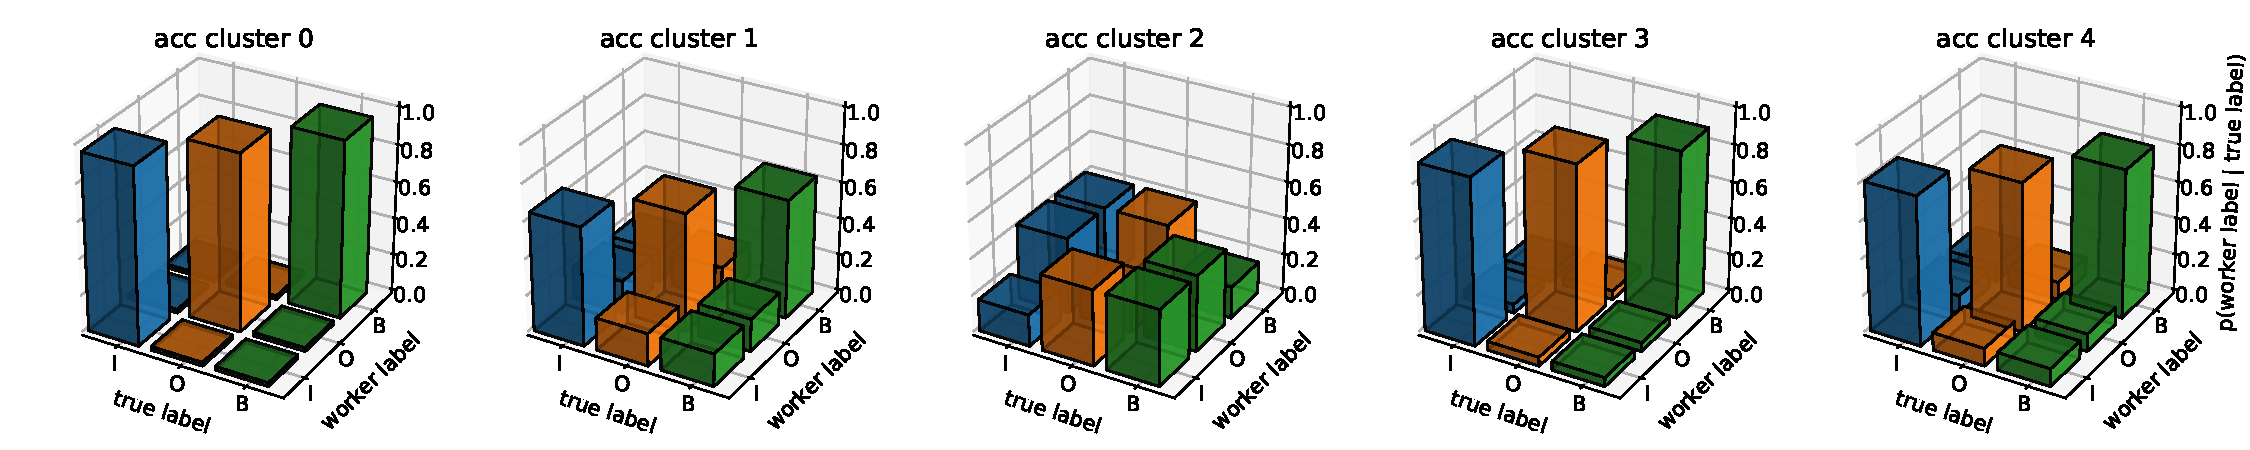
\includegraphics[width=0.9\textwidth, clip=True, trim=0 10 0 27]{figures/worker_models/acc}
% } \\
\subfloat[BSCC-Vec-IF]{
  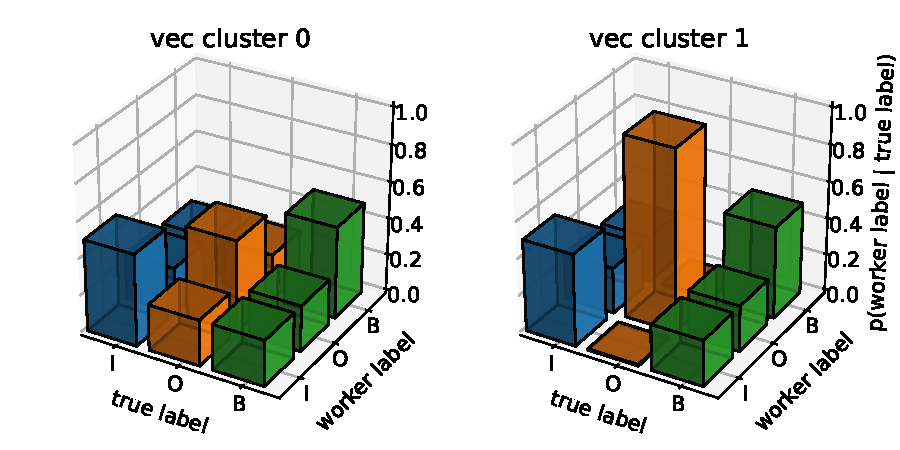
\includegraphics[width=1\textwidth, clip=True, trim=0 10 0 27]{figures/worker_models/vec}
} \\
\subfloat[BSCC-MACE-IF]{
  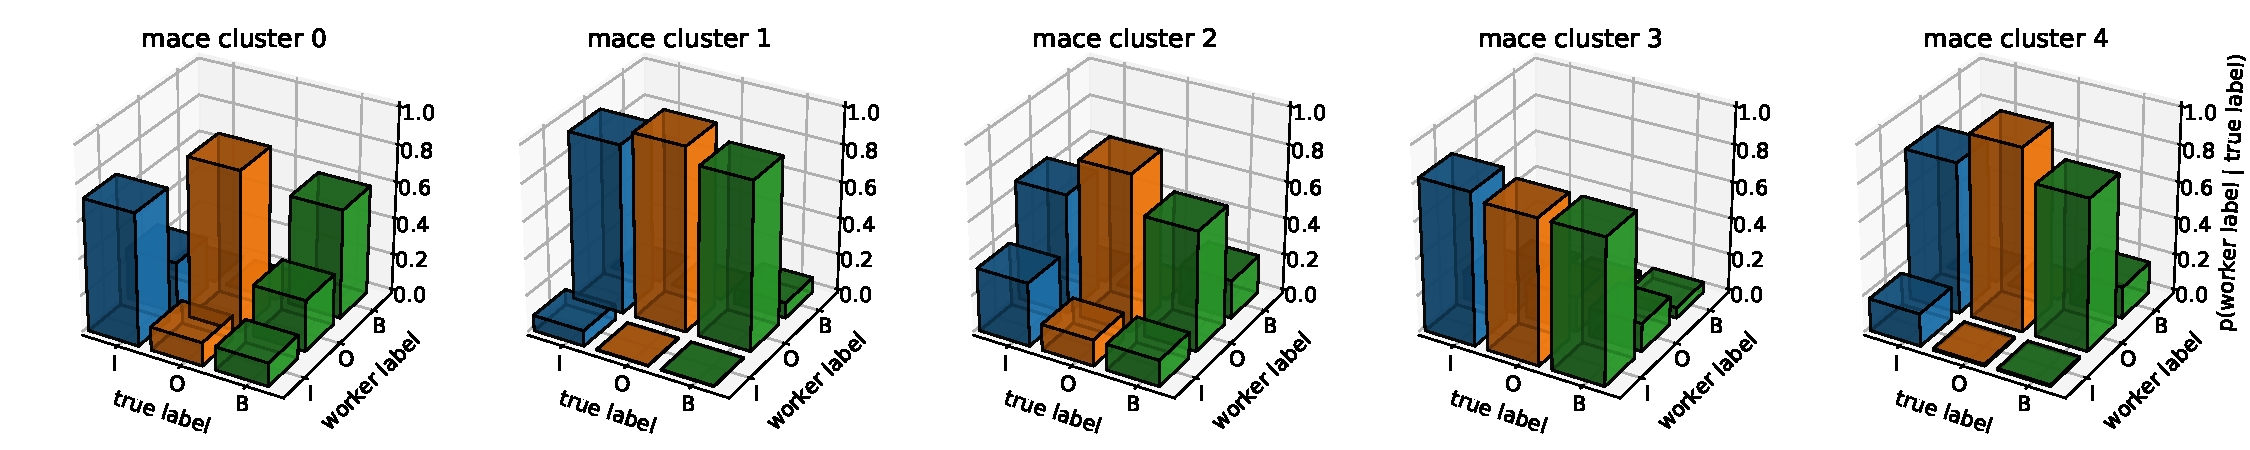
\includegraphics[width=1\textwidth, clip=True, trim=0 10 0 27]{figures/worker_models/mace}
} \\
\subfloat[BSCC-IBCC-IF]{
  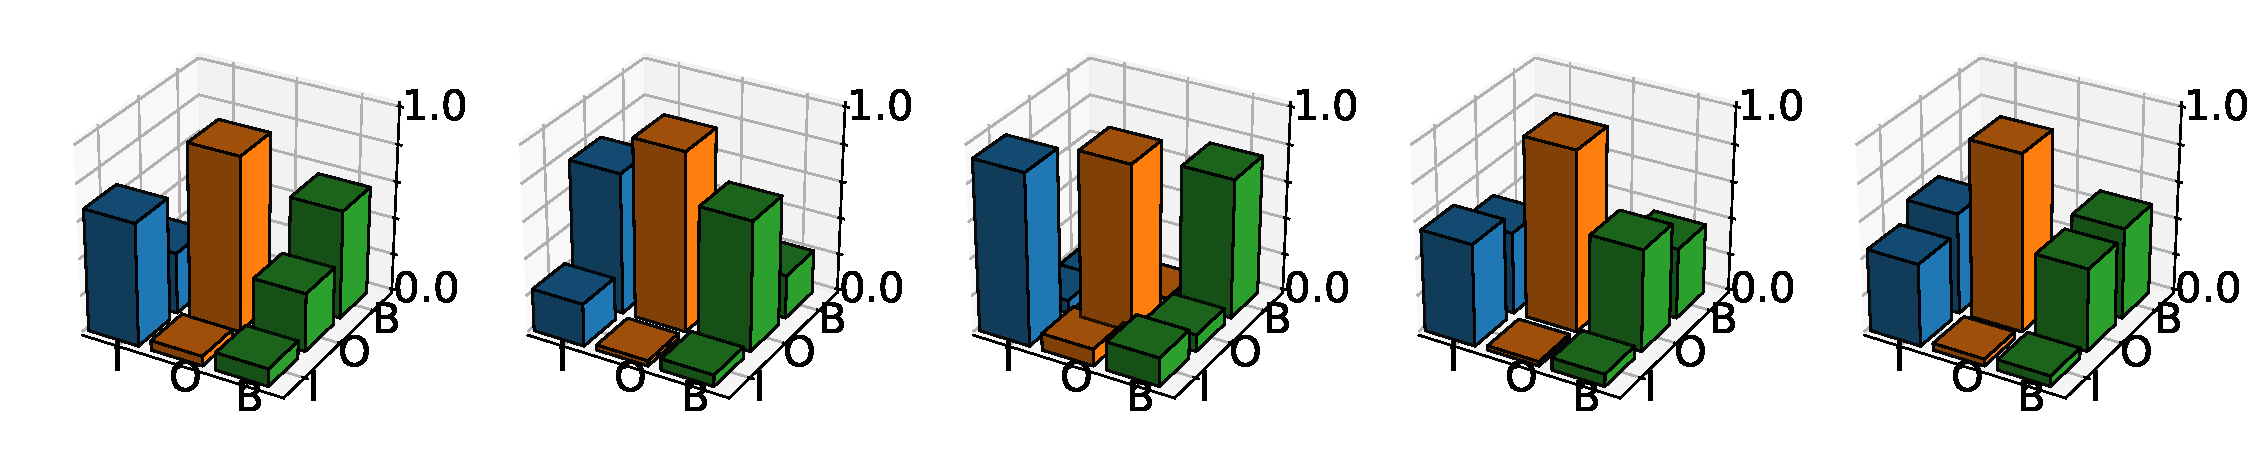
\includegraphics[width=1\textwidth, clip=True, trim=0 10 0 27]{figures/worker_models/ibcc}
} \\
\subfloat[BSCC-seq-IF, previous label = I]{
  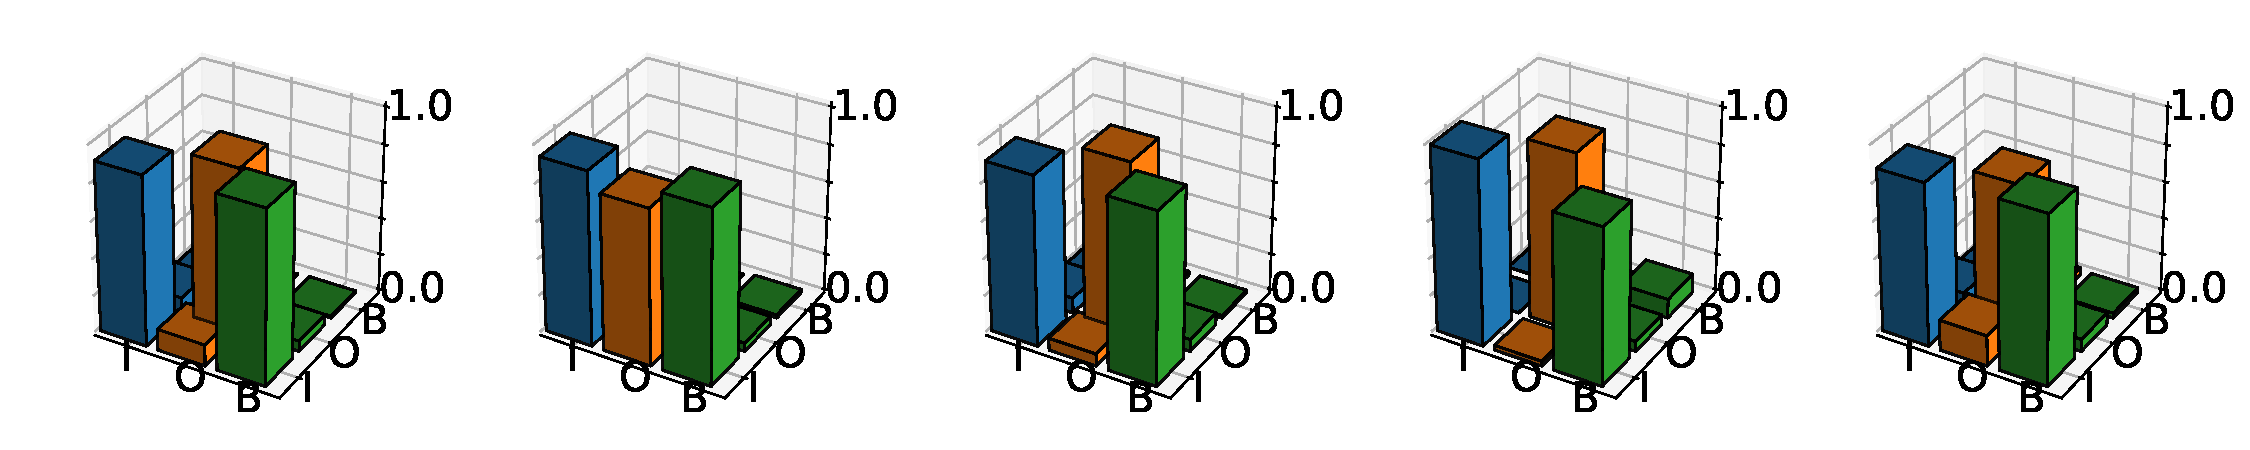
\includegraphics[width=1\textwidth, clip=True, trim=0 10 0 27]{figures/worker_models/seq_prev0}
} \\
\subfloat[BSCC-seq-IF, previous label = O]{
  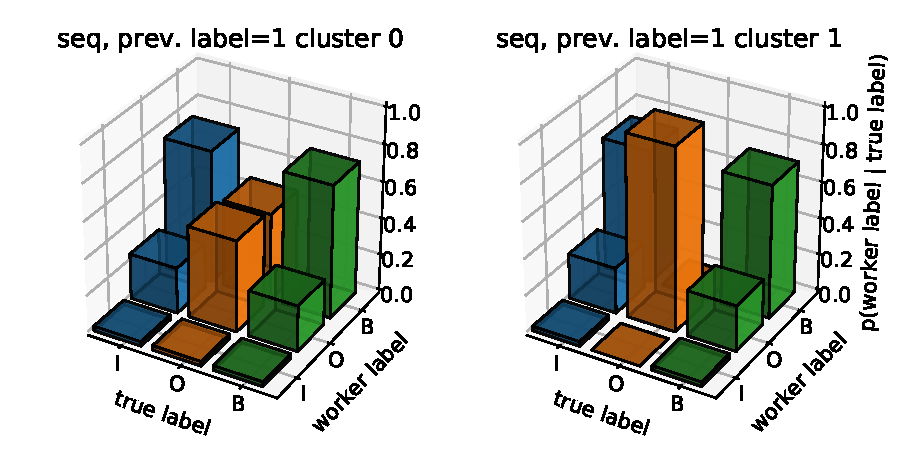
\includegraphics[width=1\textwidth, clip=True, trim=0 10 0 27]{figures/worker_models/seq_prev1}
} \\
\subfloat[BSCC-seq-IF, previous label = B]{
  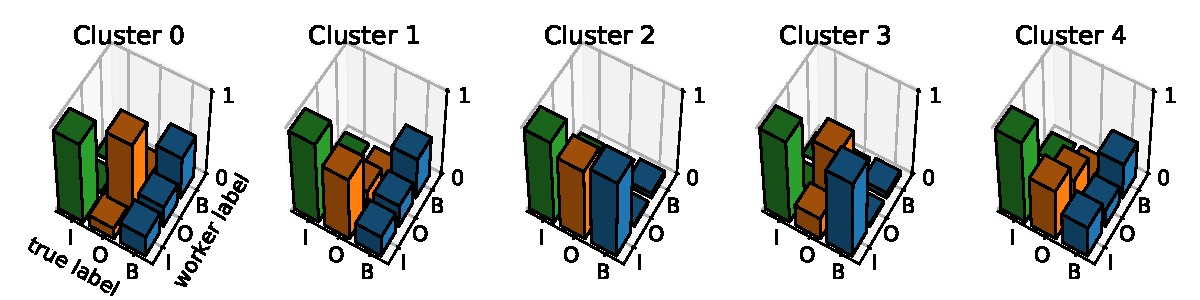
\includegraphics[width=1\textwidth, clip=True, trim=0 10 0 27]{figures/worker_models/seq_prev2}
} \\
\caption{Confusion matrix representations from each BSCC-***-IF variant trained on the PICO datasets 
showing the different representations of workers. 
% Show how worker representation benefits from richer model: e.g. show differences between rows in IBCC compared to acc.
% Represent all types as IBCC-confusion matrix plots. seq will need more >= 3 plots! We can focus on PICO data to make it easier to view,
% or combiner NER classes into BIO. 
% If each row corresponds to one model, we have 7 rows (2 extra for seq). 
% Each row can then show either a selection of 5 workers, or we can cluster into 5 groups.
}
\label{fig:conf_mat_clusters}

\end{figure*}

\begin{figure}
\centering
\subfloat[NER dataset, BSCC-IBCC-IF+LSTM]{
  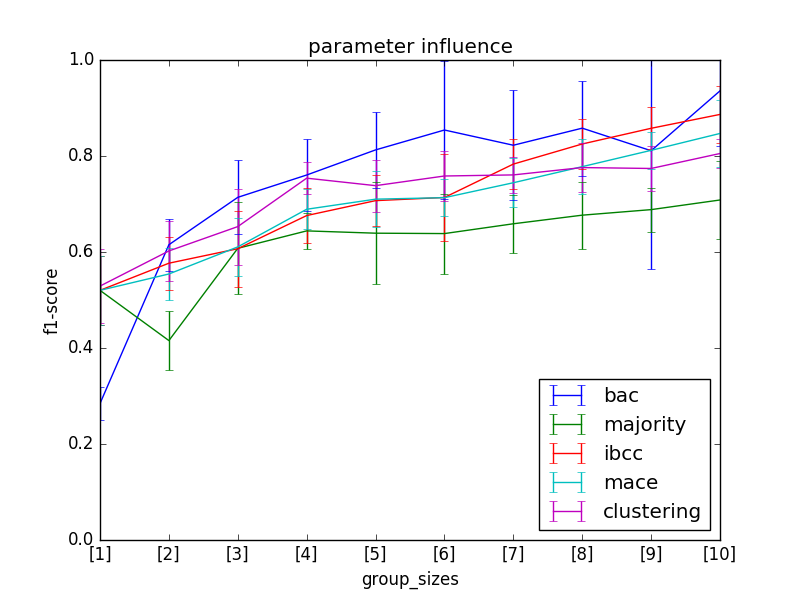
\includegraphics[width=.40\columnwidth, clip=True, trim=20 47 10 25]{figures/placeholder}
}
\subfloat[PICO dataset, BSCC-seq-IF+LSTM]{
  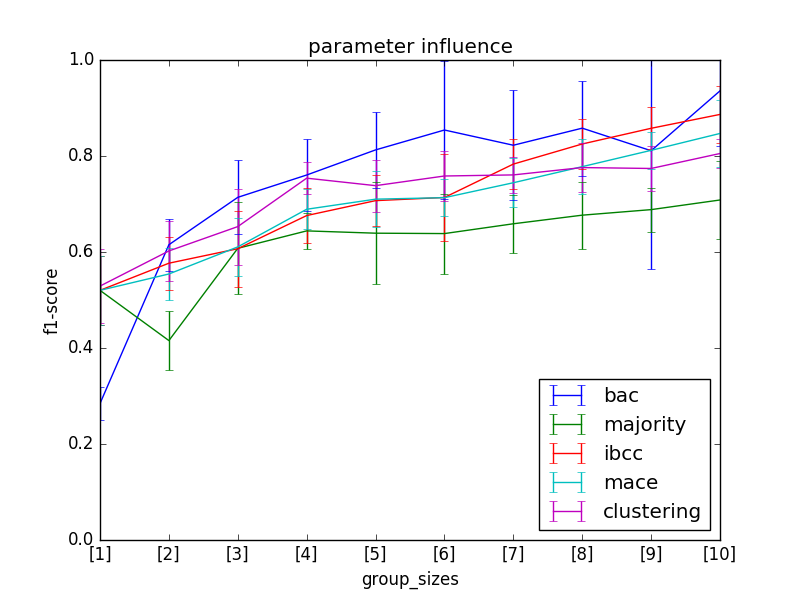
\includegraphics[width=.40\columnwidth, clip=True, trim=20 47 10 25]{figures/placeholder}
}
\caption{Confusion matrices learned for the integrated LSTM using BSCC-***-IF+LSTm. }
\label{fig:conf_mat_lstm}
\end{figure}

\subsubsection{Examples of Aggregation}

\begin{figure}
\centering
\subfloat[Example 1]{
  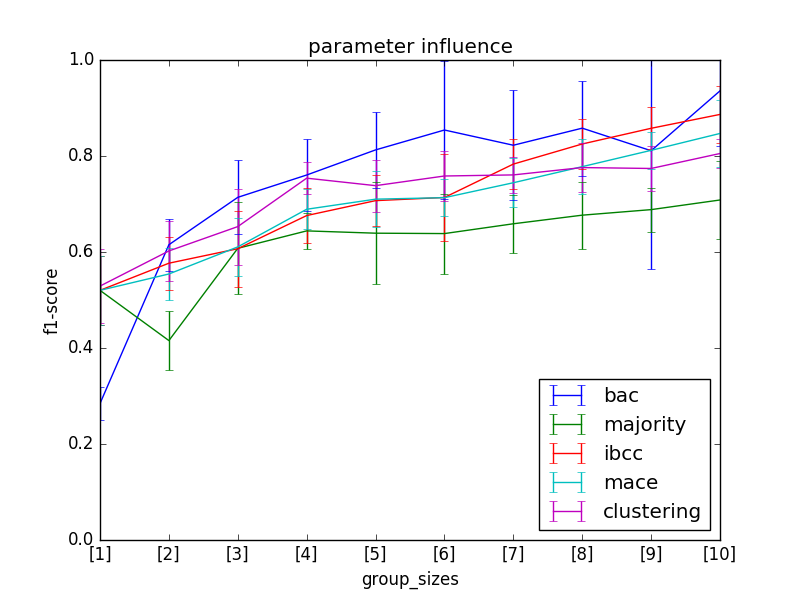
\includegraphics[width=1\columnwidth, clip=True, trim=20 47 10 25]{figures/placeholder}
}\\
\subfloat[Example 2]{
  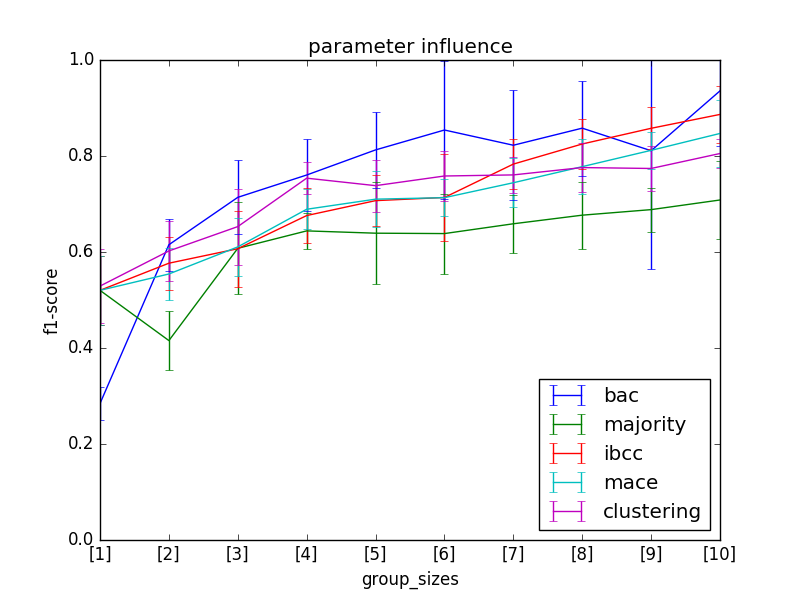
\includegraphics[width=1\columnwidth, clip=True, trim=20 47 10 25]{figures/placeholder}
}\\
\subfloat[Example 3]{
  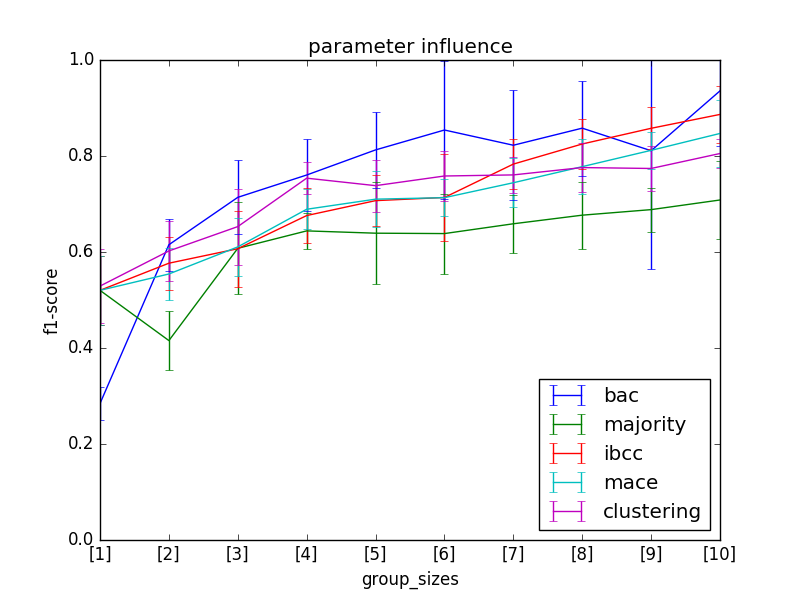
\includegraphics[width=1\columnwidth, clip=True, trim=20 47 10 25]{figures/placeholder}
}
\caption{Examples of different handling of annotator disagreement on PICO. 
Lines above the text show the crowd's annotations. Lines below show the aggregated annotations from MV, IBCC, HMM-Crowd and BSCC-seq-IF.
The sequential methods are able to resolve some issues, 
while non-sequential methods can lead to invalid annotations. }
\label{fig:disagreements}
\end{figure}

\subsection{Prediction using an LSTM Trained by the Crowd}\label{sec:task2}

In this task, we use the aggregation methods to train an LSTM sequence tagger \cite{lample2016}
to show whether integrating the LSTM with the aggregation method improves performance.
For the NER dataset, we train the aggregation methods on the $415$ crowd-labelled documents, as before,
then use the outputs to train the LSTM. We then evaluate the LSTM on the validation and test sets
in the original CoNLL dataset.
With the PICO dataset, we run the aggregators on the $3,649$ documents without gold labels, 
use the outputs to train the LSTM, then evaluate the LSTM on the validation and test splits from the gold-labelled data.


\begin{table*}
% \small
\begin{tabularx}{\textwidth}{| l | Y | Y | Y | Y | Y | Y | Y |}
\hline
NER & \multicolumn{3}{|l|}{Span-level metrics}                     & \multicolumn{4}{|l|}{Token-level metrics} \\ \hline 
& Prec. & Recall & F1 & F1 & AUC & CEE & $N_{inval}$  \\ \hline 
%HMM-Crowd-then-LSTM & 76.19 & 66.24 & 70.87 &\\ % original results from Nguyen 2017
%HMM-Crowd-then-LSTM & 72.75 & 68.26 & 70.43 & 35.73 & .8752 & 23.45 & 0 & V. close to Nguyen et al.~\shortcite{nguyen2017aggregating}\\ 
HMM-crowd$\rightarrow$LSTM & 68.8 & \textbf{65.4} & \textbf{67.1} & \textbf{67.5} & .910 & 15.21 & 1 \\ 
%LSTM & 83.19 & 57.12 & 67.73 \\ 
%LSTM-Crowd & 82.38 & 62.10 & 70.82 \\ \hline
%BSC-seq$\rightarrow$LSTM & \textbf{75.0} & \textbf{68.0} & \textbf{71.3} & \textbf{70.2} & .909 & 13.35 & 0 \\ % this was achieved before the priors were 'fixed' so that the disallowed count from banned transition from restricted_type1 -> restricted_type2 was transferred to unrestricted_type2 instead of restricted_type1. However, the method without LSTM improved...
BSC-seq$\rightarrow$LSTM & \textbf{71.5} & 59.3 & 64.9 & 66.7 & .867 & 17.43 & 0 \\  
%BSC-seq+LSTM & 71.7 & 62.7 & 66.9 & 65.9 & \textbf{.957} & \textbf{0.542} & 0 \\
BSC-seq+LSTM & 69.3 & 61.1 & 64.9 & 66.3 & \textbf{.945} & \textbf{0.89} & 0 \\  
BCC-seq+LSTM & 39.7 & 14.1 & 20.9 & 31.6 & .924 & 2.14 & 0 \\
\hline
\end{tabularx}
\caption{Prediction performance on NER test dataset with training on crowdsourced labels.}
\label{tab:prediction_results_ner}
\end{table*}

\begin{table*}
% \small
\begin{tabularx}{\textwidth}{| l | Y | Y | Y | Y | Y | Y | Y |}
\hline
PICO & \multicolumn{3}{|l|}{Span-level metrics (std.)}                          & \multicolumn{4}{|l|}{Token-level metrics (std.)} \\ \hline 
& Prec. & Recall & F1 & F1 & AUC & CEE & $N_{inval}$ \\ \hline
HMM-Crowd$\rightarrow$LSTM &\\ \hline
BSC-seq$\rightarrow$LSTM &\\
BSC-seq+LSTM &\\
BCC-seq+LSTM &\\
\hline
\end{tabularx}
\caption{Prediction performance on PICO test dataset with training on crowdsourced labels.}
\label{tab:prediction_results_pico}
\end{table*}


\section{Active Document Selection}

We run an active learning simulation to evaluate whether the proposed Bayesian approach and integrated LSTM
can improve the efficiency of the crowdsourcing process. 
The simulation is run separately for each method tested, and begins with the same initial set of randomly-chosen
documents taken from the same crowd-labelled sets used in Section \ref{sec:task2}.
We retrieve the crowdsourced labels for the selected documents, run the aggregation method,
then use its posterior probabilities to select a new batch of the $N_{batchsize}$ most uncertain documents that have not yet been labelled. 
We retrieve the annotations for the selected batch of documents, then repeat the process until
all of the availble crowd labels have been used.
We set $N_{batchsize}$ to one tenth of the crowd-labelled dataset size for each of the datasets. At each iteration,
we monitor progress by training an LSTM on the current output of the aggregation method, 
and testing its performance as in Section \ref{sec:task2}. 
With the NER dataset we also evaluate the output of aggregation method on the test set for the crowd-labelled documents. 
This is not possible with PICO datas because we do not have gold labels for documents labelled by the crowd.

The active learning process tested here employs \emph{uncertainty sampling}, which is a well-established heuristic \cite{active learning paper -- see tacl paper?}. The selection method and batch size could be fine-tuned for future applications -- the goal of our experiment in this paper was to test the benefits of the proposed aggregation methods,
rather than to establish a robust active learning approach.
 
\begin{figure*}
\centering
\subfloat[NER dataset]{
  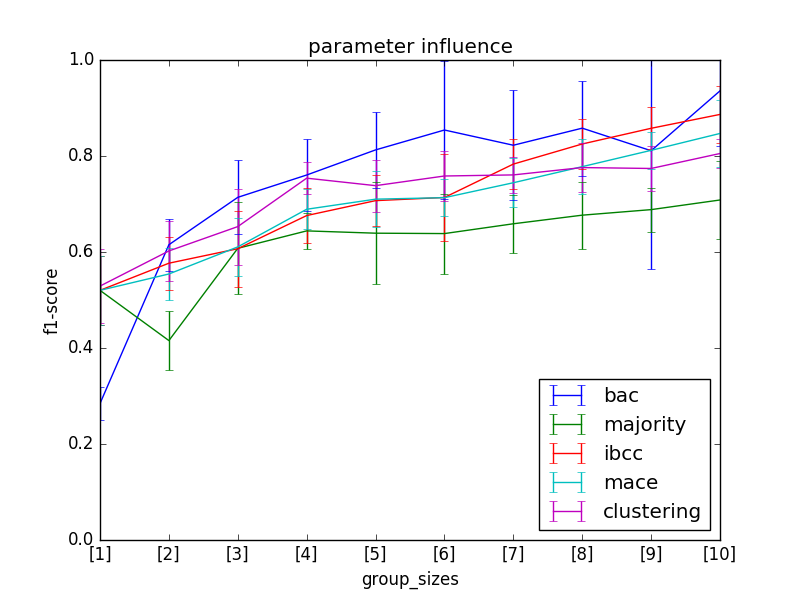
\includegraphics[width=.7\columnwidth, clip=True, trim=20 47 10 25]{figures/placeholder}
}
\subfloat[PICO dataset]{
  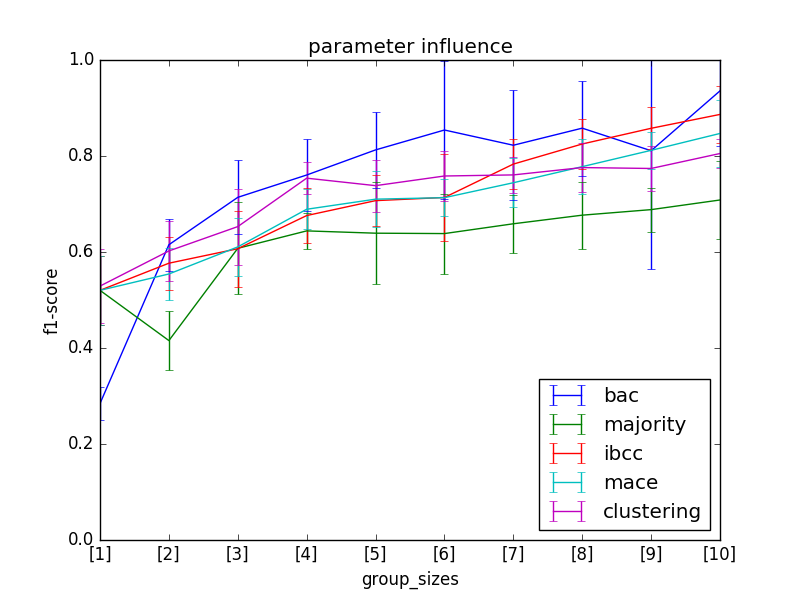
\includegraphics[width=.7\columnwidth, clip=True, trim=20 47 10 25]{figures/placeholder}
}
\caption{Active learning simulation: prediction performance after each labelled batch is received. Mean scores over 10 repeats.}
\label{fig:al}
\end{figure*}

\section{Discussion}

The benefits of sequential models are more evident on the PICO dataset than on NER, which may be due to the longer sequences or the smaller number of labels, since PICO target classes are only B, I, or O, whereas the B and I tags for NER 
are compounded with PER, LOC, ORG or MISC tags. <show an example from each dataset, with our predictions from HMM, BAC...>

\section{Conclusions}

Previous work has demonstrated the benefits of modeling annotator reliability when aggregating noisy data, 
such as crowdsourced labels. 
We proposed a sequential annotator model for sequence tagging, BSC-Seq,
and showed how it improves the state-of-the-art. 
%To enable more efficient training data collection,
To further improve the quality of aggregated labels,
we design a Bayesian wrapper that allows developers to integrate existing sequence taggers, 
such as deep neural networks, into BSC-Seq while
treating them as black boxes.
Our results show that integrating an LSTM in this manner can outperform an LSTM trained 
using labels that were aggregated in a separate pre-processing step. 
However, for active learning from crowds or learning with small datasets, 
we find that our purely Bayesian aggregation method, i.e. BSC-Seq without integrating the LSTM,
outperforms both LSTM-based approaches. This hints at the value of uncertainty information
in text models when data-efficient learning is required. 

Future work will investigate the integration of approximate Bayesian variants of neural network
sequence taggers, which may address the need for uncertainty information during active learning.
We will also consider
%  improving robustness of the active learning process with very small datasets by investigating 
alternative data selection strategies, and how to include %reduce over-confidence in predictions by including
prior information about the reliability of black-box classifiers on a given training set size.

%how to adapt hyper-parameters of the NN automatically in low-resource state?

% % In future, BSC-Seq could be applied to other sequential classification tasks beside span annotation.
% For example, the order of tasks that are intended to be exchangeable may affect the likelihood
% of the labels provided by the annotators\cite{mathur2017}. Seq-BCC could be applied to model the 
% propensity of the workers to choose certain labels given their previous labels, while the 
% ground truth sequence may be ignored.


%%%%%%%%%%%%%%%%%%%%%%%%%%%%%%%%%%%%%%%%%%%%%%%%%%%%%%%%%%%%%%%%%%%%%%%%%%%%%%%%

\section*{Acknowledgments}

This work was supported by the German Research Foundation through the German-Israeli Project Cooperation (DIP, grant DA 1600/1-1 and grant GU 798/17-1), and 
by the German Research Foundation (DFG) as part of the QA-EduInf project (grant GU 798/18-1 and grant RI 803/12-1). 

% \addcontentsline{toc}{chapter}{Bibliography}
%\bibliographystyle{apalike}
% \bibliographystyle{IEEEtran}
\bibliographystyle{acl_natbib}
\bibliography{simpson}

\appendix
\section{Discussion of Variational Approximation}

In Equation 12 of the main paper,
each subset of latent variables has a variational factor of the form 
$\ln q(z) = \mathbb{E}[\ln p(z | \bs c, \neg z)]$, 
where $\neg z$ contains all the other latent variables excluding $z$.
We perform approximate inference by
%we optimize Equation \ref{eq:vb_posterior} 
using coordinate ascent to update each variational factor, $q(z)$, in turn,
taking expectations with respect to the current estimates of the other variational factors.
%(see Algorithm \ref{al:vb_bac}).
Each iteration reduces the KL-divergence between the true and approximate posteriors
of Equation 12, and hence optimises a lower bound on the 
log marginal likelihood, also called the evidence lower bound or ELBO
~\cite{Bishop2006,attias_advances_2000}.

\paragraph{Conjugate distributions: }The prior distributions chosen for our generative model are conjugate to the distributions over the
latent variables and model parameters, 
meaning that each $q(z)$ is the same type of distribution
as the corresponding  prior distribution defined in Section 4.
The parameters of each variational distribution are computed in terms  of 
expectations over the other subsets of variables.


\begin{figure*}[t]
\begin{minipage}[b][1cm][l]{0.2\textwidth} 
BSC-seq, \\
previous label = I:
\end{minipage}
  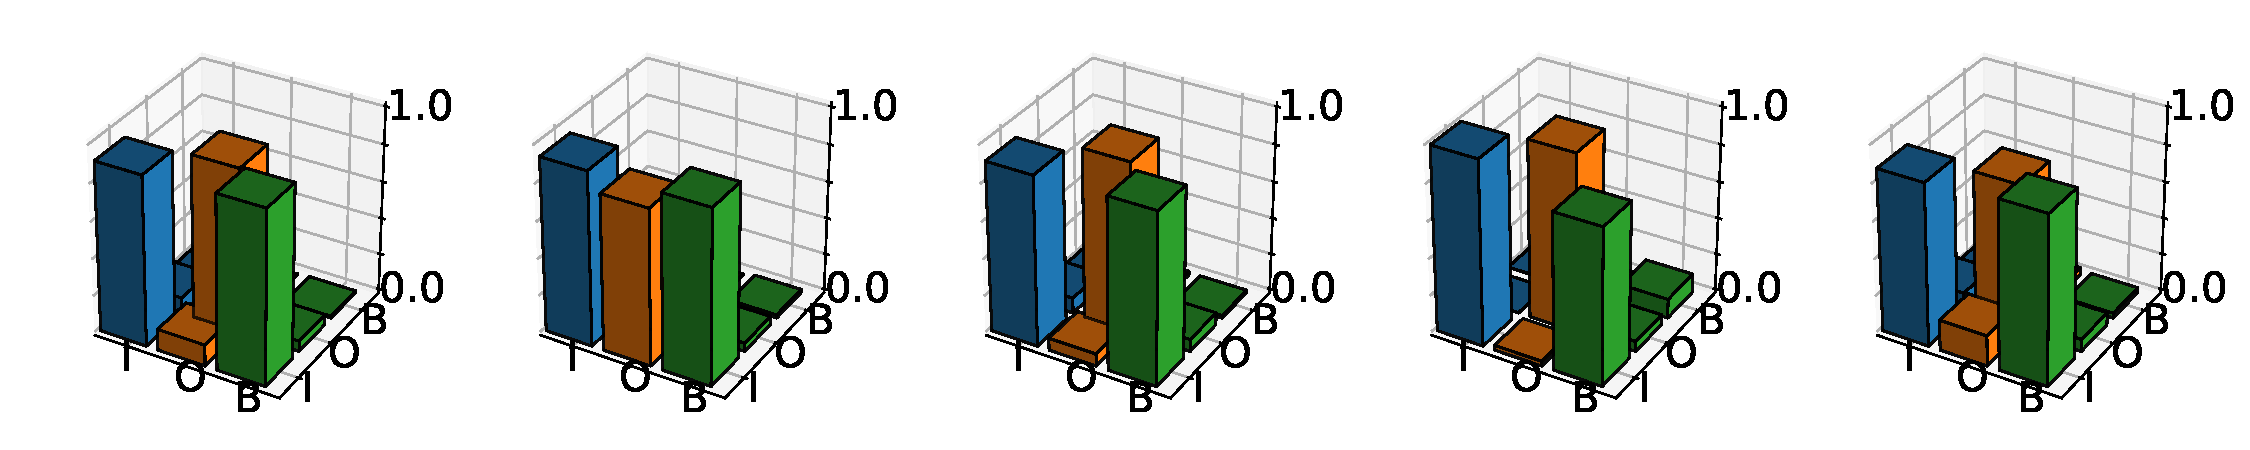
\includegraphics[width=0.8\textwidth, clip=True, trim=10 0 0 10]{figures/worker_models/seq_prev0}
\\
\begin{minipage}[b][1cm][l]{0.2\textwidth} 
BSC-seq, \\
previous label = O:
\end{minipage}
  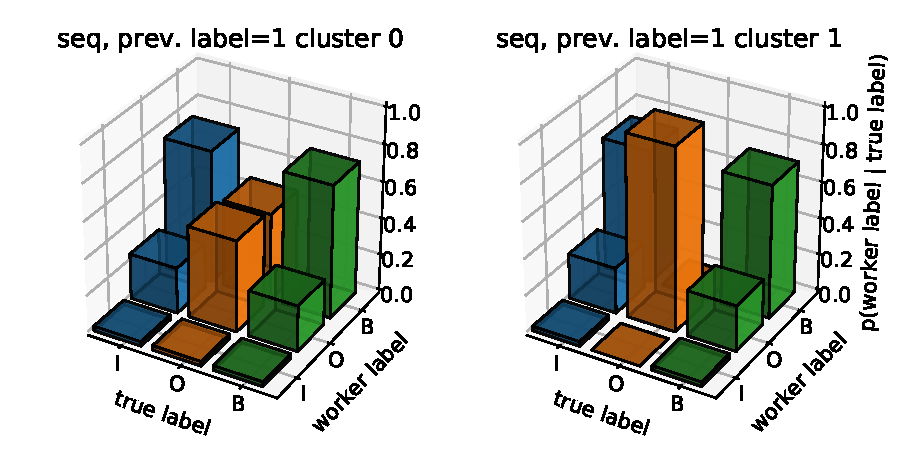
\includegraphics[width=0.8\textwidth, clip=True, trim=10 0 0 23]{figures/worker_models/seq_prev1}
\\
\begin{minipage}[b][1cm][l]{0.2\textwidth} 
BSC-seq,\\
 previous label = B:
\end{minipage}
  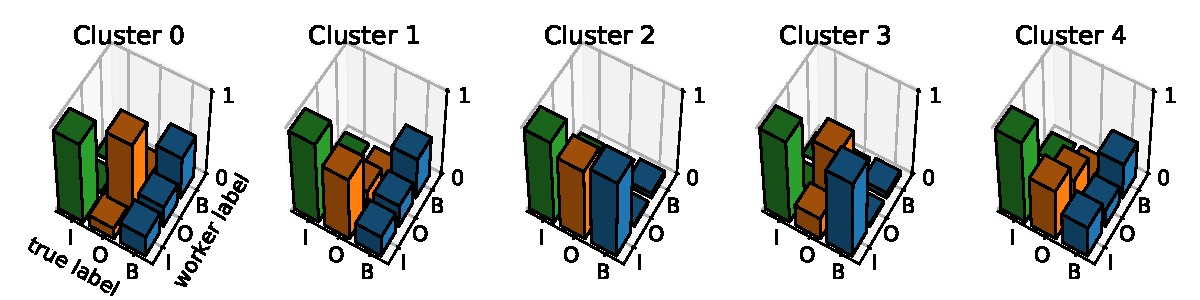
\includegraphics[width=0.8\textwidth, clip=True, trim=10 0 0 23]{figures/worker_models/seq_prev2}
\\
\caption{Clusters of confusion matrix representations from BSC-seq trained on PICO. 
}
\label{fig:anno_models_2}
\end{figure*}

\section{Update Equations for the Forward-Backward Algorithm}

For the true labels, $\bs t$, the variational factor is:
 \begin{flalign}
& \ln q(\bs t_n) \!=\! 
% \sum_{n=1}^N \sum_{\tau=1}^{L_n} 
% \sum_{s=1}^S \mathbb{E}%_{\bs B,\bs d^{(s)}} \!\left[ 
% \ln \!B^{(s)}\!\!\left(t_{n,\tau},d_{n,\tau}^{(s)},d_{n,\tau\!-\!1}^{(s)}\!\right) %\right]
% %\bigg\{ \mathbb{E}%_{\bs T} \left[ 
% %\ln T_{t_{n,\tau\!-\!1}, t_{n,\tau}} %\right] 
% &&\nonumber \\
%+ 
\sum_{n=1}^N \sum_{\tau=1}^{L_n} \sum_{k=1}^K  \mathbb{E}%_{\bs A} \left[ 
\ln \!A^{(k)}\left(t_{n,\tau},c_{n,\tau}^{(k)},c_{n,\tau-1}^{(k)}\right) %\right]  
&\nonumber\\
&+ \mathbb{E}\ln T_{t_{n,\tau-1}, t_{n,\tau}}+\mathrm{const}. & \label{eq:qstar_t}
 \end{flalign}
 
% TODO move all this to the appendix
 The forward-backward algorithm consists of two passes. 
 The \emph{forward pass} for each document, $n$, starts from $\tau=1$
 and computes:% for each value of $\tau$:
 % the posterior given crowdsourced annotations for tokens $\leq\tau$. 
 \begin{flalign}
   & \ln r^{-}_{n,\tau,j} = \ln \sum_{\iota=1}^J \left\{ r^{-}_{n,\tau-1,\iota} \mathrm{e}^{\mathbb{E}\ln T_{\iota,j}} \right\} + ll_{n,\tau}(j), & \nonumber \\
% \end{flalign}
%  where the log likelihood $ll(j,n,\tau)$ of the annotations for token $\tau$ in document $n$ giventr
%  label $j$ is:
% \begin{flalign} 
   & ll_{n,\tau}(j) = \sum_{k=1}^K \mathbb{E}%_{\bs A}
   \ln A^{(k)}\left(j, c_{n,\tau}^{(k)}, c_{n,\tau\!-\!1}^{(k)} \right) & 
   %+  \sum_{s=1}^S
%    & \nonumber \\
%    &  \sum_{i=1}^J\sum_{\iota=1}^J \mathbb{E}%_{\bs B}
%    \ln B^{(s)} \!\left(j, i, \iota \right)  
%    \hat{d}_{n,\tau}^{(s)}(i) \hat{d}_{n,\tau-1}^{(s)}(\iota), & 
 \end{flalign}
 %where $\hat{d}_{n,\tau}^{(s)}(i)$ is %the probability of label $d_{n,\tau}^{(s)}$ produced 
% by the sequence tagger $s$, which we explain in more detail below (see Equation \ref{eq:hatp}).
%defined below in Equation \ref{eq:hatp}, and 
where $r^{-}_{n,0,\iota}  = 1$ where $\iota=$`O' and $0$ otherwise.
The \emph{backwards pass} starts from $\tau=L_n$ and scrolls backwards, computing:
%at each token computing the likelihoods of the annotations from $\tau+1$ to $L_n$:
 \begin{flalign}
  & \ln \lambda_{n,L_n,j} = 0, \hspace{1cm}
   \ln \lambda_{n,\tau,j} = \ln\sum_{\iota=1}^J \exp \big\{ 
   & \nonumber \\
& \ln \lambda_{i,\tau+1,\iota} + \mathbb{E}\ln T_{j,\iota} + ll_{n,\tau+1}(\iota) \big\} .&
 \end{flalign}
% To avoid $r^{-}_{n,\tau,j}$ and $\lambda_{n,\tau,j}$ becoming too small over a long sequence, we normalize them after each iteration of the forward and backward pass
% by dividing by their sum over $j$.
 By %taking the exponents and 
 applying Bayes' rule, we arrive at $r_{n,\tau,j}$ and $s_{n,\tau,j,\iota}$:
 \begin{flalign}
  & r_{n,\tau,j} = \frac{r^{-}_{n,\tau,j}\lambda_{n,\tau,j}}{\sum_{j'=1}^J r^{-}_{n,\tau,j'}\lambda_{n,\tau,j'}} &\\
%} {\sum_{\iota=1}^J \sum_{\iota'=1}^J  
%  r^{-}_{n,\tau\!-\!1,\iota}\lambda_{n,\tau,\iota'} \exp\mathbb{E}[\ln T_{\iota,\iota'}] 
% + ll(\iota',n,\tau)  } . &
& s_{n,\tau,j,\iota} = \frac{ \tilde{s}_{n,\tau,j,\iota} }{ \sum_{j'=1}^J\sum_{\iota'=1}^J  \tilde{s}_{n,\tau,j',\iota'} } & \\
  & \tilde{s}_{n,\tau,j,\iota} =  r^{-}_{n,\tau-1,j} \lambda_{n,\tau,\iota} \exp\{\mathbb{E}\ln T_{j,\iota}
+ ll_{n,\tau}(\iota)\}. & \nonumber 
 \end{flalign}
 
 Each row of the transition matrix has the factor:
\begin{flalign}
& \ln q(\bs T_{j}) 
  %= \sum_{\iota=1}^J N_{j,\iota}  + \ln \mathrm{Dir}(\bs T_j | \bs\gamma_j) + \mathrm{const} & \nonumber\\
= \ln \mathrm{Dir}\left(\left[ N_{j,\iota} + \gamma_{j,\iota}, \forall \iota \in \{1,..,J\} \right]\right), &
\end{flalign}
where $N_{j,\iota} = \sum_{n=1}^N \sum_{\tau=1}^{L_n}  s_{n,\tau,j,\iota}$ is the expected number of times that label $\iota$ follows label $j$.  
%The variational factor $q(\bs t)$ requires the following expectation:
The forward-backward algorithm requires expectations of $\ln \bs T$ that can be computed using standard equations for a Dirichlet distribution:
 \begin{flalign}
& \mathbb{E}\ln T_{j,\iota} = \Psi\!\left(N_{j,\iota} \!\!+ \gamma_{j,\iota}\right) 
 - \Psi\!\left(\sum_{\iota=1}^J (N_{j,\iota} \!\!+ \gamma_{j,\iota}) \!\right), &
\end{flalign}
 where $\Psi$ is the digamma function.
 
 
 
%\textbf{Variational factors for} $\bs A$ and $\bs B$:
The variational factor for each annotator model is a distribution over its parameters, 
which differs between models.
For \emph{seq}, the variational factor is:
 \begin{flalign}
  & \ln q\!\left(\! A^{(k)}\!\right) %= \sum_{j=1}^J  \sum_{l=1}^J \bigg\{ \sum_{m=1}^J N_{j,l,m}^{(k)}\ln\pi_{j,l,m}^{(k)} & \nonumber\\
 % & \hspace{2.7cm} 
 % + \ln p\left(\bs\pi_{j,l}^{(k)} | \bs \alpha_{j,l}^{(k)} \right) \bigg\} + \mathrm{const}, & \nonumber \\
  \!=\! \sum_{j=1}^J \! \sum_{l=1}^J \!\mathrm{Dir}\! \left(\left[ \bs N_{j,l,m}^{(k)} \! 
 %+ \alpha_{j,l,m}^{(k)}, \! 
 %\right.\right.\nonumber&\\
%&  \hspace{3.5cm} \left.\left.
\forall m \! \in \! \{1,..,J\} \!\right] \right) & \nonumber \\
& N^{(k)}_{j,l,m} \!\!=\!  \alpha_{j,l,m}^{(k)} \!\!\! + \!\sum_{n=1}^N \!\sum_{\tau=1}^{L_n} \!
r_{n,\tau,j} \delta_{l,c^{(k)}_{n,\tau\!-\!1}}\!\delta_{m,c^{(k)}_{n, \!\tau}}, \!& 
\end{flalign}
 where $\delta$ is the Kronecker delta. 
% For the \emph{CM} model, the variational factor is simplified to:
%  \begin{flalign}
%   & \ln q\left( A^{(k)}\right) = \sum_{j=1}^J  \mathrm{Dir} \bigg( \bigg[ \sum_{n=1}^N \sum_{\tau=1}^{L_n} r_{n,\tau,j} \delta_{m,c^{(k)}_{n,\tau}} 
%   & \nonumber \\ 
% & \hspace{2.0cm} + \alpha_{j,m}^{(k)}, \! \forall m \! \in \! \{1,..,J\} \bigg] \bigg) .
% \end{flalign}
For \emph{CM}, \emph{MACE}, \emph{CV} and \emph{acc}, the factors follow a similar pattern of summing pseudo-counts of correct and incorrect answers. 
%For reasons of space, we omit the equations for these variants. 

\section{Visualising Annotator Models}

Figure \ref{fig:anno_models_2} provides an alternative visualisation of the \textit{seq} models inferred by BSC-seq for annotators in the PICO dataset.
The annotators were clustered as described in Section 6 of the main paper,
and the mean confusion matrices for each cluster are plotted in Figure \ref{fig:anno_models_2} using 3D plots to emphasise the differences between 
the likelihoods of annotators in each cluster providing a particular label 
given the true label value.

\end{document}
